\documentclass[useAMS, usenatbib]{mnras}
\pdfsuppresswarningpagegroup=1
%
\usepackage[spanish,es-minimal,english]{babel}
\usepackage[utf8]{inputenc}
\usepackage{graphicx}

\usepackage{xcolor}
\usepackage{hyperref}
\usepackage{siunitx}
\usepackage{newtxtext}
\usepackage[stix2,smallerops]{newtxmath}
\usepackage{booktabs}
\hypersetup{colorlinks=True, linkcolor=blue!50!black, citecolor=black,
  urlcolor=blue!50!black}
\usepackage{etoolbox}
\robustify\bfseries
\robustify\itshape

\bibliographystyle{mnras}

\sisetup{
  % explicit "+" is useful for velocities
  retain-explicit-plus = true,
  % prefer 10^6 over 1 x 10^6
  retain-unity-mantissa = false,
  % Use x +/- e instead of x(e)  
  separate-uncertainty = true,
  % Make sure to pick up bold font when used in section heading for instance
  detect-weight = true,
}
\DeclareSIUnit\msun{\text{\ensuremath{M_\odot}}}

%%
%% Will macros
%%
% A better \ion command that works in more circumstances
\newcommand\ION[2]{#1\,\scalebox{0.9}[0.8]{\uppercase{#2}}}
\newcounter{ionstage}
\renewcommand{\ion}[2]{\setcounter{ionstage}{#2}% 
  \ensuremath{\mathrm{#1\,\scriptstyle\Roman{ionstage}}}}
\newcommand\hii{\ion{H}{2}}
\newcommand\nii{[\ion{N}{2}]}
\newcommand\oiii{[\ion{O}{3}]}
\newcommand\oii{[\ion{O}{2}]}
\newcommand\Wav[1]{\ensuremath{\lambda #1}}
% Chemical formulae
\newcommand*\chem[1]{\ensuremath{\mathrm{#1}}}


%%
%% Teresa macros
%%
\newcommand{\Sub}[1]{_\mathrm{#1}}
\newcommand{\SSub}[1]{_\mathrm{\scriptscriptstyle #1}}
\newcommand{\Sup}[1]{^\mathrm{#1}}
\newcommand{\kms}{\ensuremath{\mathrm{km\ s}^{-1}}}
\newcommand{\pcc}{\ensuremath{\mathrm{cm}^{-3}}}
\newcommand{\sii}{[\ion{S}{2}]}
\newcommand{\heii}{\ion{He}{2}}
\newcommand\OIlam{[\ion{O}{1}]\,6300\,\AA\@}
\newcommand\SIIlam{[\ion{S}{2}]\,6731\,\AA\@}
\newcommand\SIIlamshort{[\ion{S}{2}]\,6716\,\AA\@}
\newcommand\SIIlamboth{[\ion{S}{2}]\,6716,6731\,\AA\@}
\newcommand\SIIIlam{[\ion{S}{3}]\,6312\,\AA\@}
\newcommand\NIIlam{[\ion{N}{2}]\,6583\,}
\newcommand\NIIlamlam{[\ion{N}{2}]\,6548,6584\,\AA\@}
\newcommand\OIIIlam{[\ion{O}{3}]\,5007\,\AA\@}
\newcommand\HeIIlam{HeII\,4686\,\AA\@}
\newcommand\Halam{H$\alpha$\,6563\,\AA\@}
\newcommand\Ha{\ensuremath{\mathrm{H}\alpha}}
\newcommand\Hb{\ensuremath{\mathrm{H}\beta}}
\newcommand{\vhel}{\ensuremath{V_\mathrm{hel}}}
\newcommand{\vmean}{\ensuremath{\langle V\rangle}}
\newcommand{\vsys}{\ensuremath{V_\mathrm{sys}}}
\newcommand{\vexp}{\ensuremath{V_\mathrm{exp}}}
\newcommand{\hr}{\ensuremath{^\mathrm{h}}}
\newcommand{\minute}{\ensuremath{^\mathrm{m}}}
\newcommand{\teff}{\ensuremath{T_\mathrm{eff}}}


\title{The complex structure and peculiar internal motions of the planetary nebula NGC 6210}

\author[López et al.]{
  William J. Henney,\(^1\)\thanks{
    w.henney@irya.unam.mx,
    jal@astro.unam.mx,
    tere@astro.unam.mx,
    richer@astro.unam.mx
  }
  J. A. López\(^2\)\footnotemark[1]
  Ma.\ T. García-Díaz,\(^2\)\footnotemark[1]
  and M. G. Richer\(^2\)\footnotemark[1]
  \\
  \(^1\)\foreignlanguage{spanish}{
    Instituto de Radioastronomía y
    Astrofísica, Universidad Nacional Autónoma de México, Apartado
    Postal 3-72, 58090 Morelia, Michaoacán, Mexico}
  \\
  \(^2\)\foreignlanguage{spanish}{
    Instituto de Astronomía,
    Universidad Nacional Autónoma de México,
    Ensenada, Baja California, 22800, México}
}
% These dates will be filled out by the publisher
\date{Accepted XXX. Received YYY; in original form ZZZ}

% Enter the current year, for the copyright statements etc.
\pubyear{2020}




\begin{document} 
\label{firstpage}
\pagerange{\pageref{firstpage}--\pageref{lastpage}}
\maketitle

\begin{abstract}
  A comprehensive kinematic study has been carried out on the planetary nebula (PN) NGC 6210. Multiple long-slits, echelle spectra have been obtained over the face of this nebula mapping its full shell structure, the opposite pairs of extended, twisted arms and the bipolar collimated outflows and bullets. Public {\it HST} imagery has been used to identify kinematic elements with structural components. The long-slit spectroscopic information has been combined into channel maps that greatly facilitate visualizing the otherwise intricate expansion pattern of this  planetary nebula. The global morphology of NGC 6210 is  reminiscent of other planetary nebulae with extended X-ray emission, suggesting the presence of a central hot bubble produced by shocked stellar wind. In spite of the dramatic structure of this PN substantial expanding radial motions are only found in the material surrounding the central, inner shell. The relatively slow radial motions of the collimated outflows and the bullet-like knots indicate that they are  moving away from the core very close to the plane of the sky, nearly perpendicular to the line of sight. The direction and ages of the various components, derived from their expanding velocities indicate that NGC 6210 has been strongly influenced by the  action of a bipolar, rotating, episodic outflow.
\end{abstract}


\begin{keywords}
  Planetary Nebulae: individual (NGC~6210)
  -- ISM: kinematics and dynamics -- ISM blowout
  -- techniques: imaging spectroscopy
\end{keywords}

\maketitle

\section{INTRODUCTION}
\label{sec:introduction}
NGC 6210 is a bright and relatively large PN in the northern sky. The first photographic image of NGC 6210 was published by \citet{Duncan:1937a}. In that old, fuzzy image a pair of twisted arms protruding in opposite directions from a blurred,  bright, nebular core are apparent. Several studies have discussed the inner kinematic motions of this object, e.g. \citet{Osterbrock:1966a, Weedman:1968a, Becker:1984a, Icke:1989a}. However, none of those studies had the spatial coverage and spectral resolution needed to produce a reliable spatio-kinematic model of this PN. 
The best kinematic study to date on NGC 6210 is probably the one published by \citet{Phillips:1996a}  who obtained 11 long-slits centered on the nebular core, with each slit at different position angles thus providing a good spatial coverage but with only limited, low and medium spectral resolution. From these data they suggested a reasonable, though somewhat basic, kinematic model for the ionized nebula. NGC 6210 jumped into fame thanks to the {\it HST} images obtained during the 1996 - 1998 period under the observing programs 6347 (K. Borkowski), 6792 (R. Rubin), 7501 (A. Hajian)  and 11122 (B. Balick). These images showed for the first time the extraordinarily complex morphology of NGC 6210. Incidentally the  {\it HST} and ground-based imagery prompted the nickname "the turttle" for this nebula, given the shape of its main body and extended arms that resemble the shell of a turttle with a long neck and its fins. The distance estimates to NGC 6210 vary roughly from 1.5 to 2.0 kpc. \citep{Hajian:1995a} derive a distance to NGC 6210 from VLA 6 cm  expansion parallax measurements of 1.57$\pm0.40$ kpc, considering an expansion velocity of 23 \kms, whereas Frew (20XX) derives a distance of kpc to this object from its H$\alpha$ surface brightness method.

In this work we present a thorough spectral mapping of all the morphological elements of the PN obtained at high spectral resolution that allow 
disentangling the various spatio-kinematic components and provide an overall view of its structure and evolution. Radial velocities are combined with 2-epoch HST \oiii ~and~ \nii ~archive image sets (http://archive.stsci.edu/) to derive proper motions. Individual long-slit echelle spectra obtained over 5 observing runs are analyzed as position - velocity data and combined into emission and velocity channel maps that serve as an excellent tool to visualize and understand the peculiar velocity fields, of the several structural components.

In Section 2, we describe our observations and the data-reduction steps, In Section 3 we describe the proper motions, In Section 4, we discuss the kinematic components from slit spectra. In next section, we present the dynamical ages and finally in section 5 we present the discussion and conclusion. 

\section{OBSERVATIONS AND DATA REDUCTION}
\label{sec:observations}

Long-slit, echelle, spectroscopic observations of the nebula NGC~6210
were performed with the 2.1~m telescope at the Observatorio
Astron\'omico Nacional at San Pedro M\'artir, (OAN-SPM), Baja
California, M\'exico. We used the Manchester Echelle Spectrometer
(MES-SPM) \citep{Meaburn:2003a} on the 2.1 m telescope in its $f$/7.5
configuration.  The MES-SPM is a long-slit, echelle spectrometer that
has no cross-disperser; it isolates single orders using interference
filters. We used a 90\,\AA\, and 50\,\AA\, bandwidth
filter to isolate the 87th and 114th orders containing the
\Ha\,$+$\,\NIIlam\, and \OIIIlam\, nebular emission lines,
respectively. Spectroscopic data on NGC 6210 was collected within our regular observing programs over nine observing runs from 1998 till 2019. Table 1 shows the log of observations. In the first column the dates for the individual observing runs are listed; the second column lists the exposure times mostly used in the corresponding run; the third column lists the spectral range of the observations, namely, $H\alpha$ + [N II] and/or [O III]; the fourth column lists the slit width in microns and the fifth column the position angle of the slit. Finally, in the sixth column the nomenclature used to identify the slits obtained in each run is indicated. In the end 34 slit positions from all the runs were selected to analyse the kinematic structure of NGC 6210. The location of these slits are presented and labeled against an [N II] $\rm HST$ archive image in Figure 1. In the top panel the vertical solid lines represent the set of 11 slits obtained in the 2015 run. The vertical dashed lines represent 12 slit positions from other runs, in some cases they are highly coincident in location with the 2015 set but selected for reasons such as different exposure times or spectral range. The middle panel shows 5 slit positions oriented E - W and the bottom panel 6 slit positions obtained at an angle intended to record specific features, such as collimated outflows or the twisted arms of the nebula. In order to establish the exact position of the slit in each pointing, the slit position on the sky was recorded with an automatic procedure available in MES-SPM prior to the spectroscopic exposure.

During the 11 years span of the observations different detectors were used with MES. Their general characteristics are described below

A TEK-1 CCD detector was used for the 1998 data set with 1024 $\times$ 1024 square pixels, each 24$\mu$m on a side, $\equiv$0.312 arcsec pixel$^{-1}$. A 2$\times$2 binning was set, consequently, 512 increments, each 0\farcs624{} long gave a projected slit length of 5\farcm32 on the sky. For slits 150 $\mu$m ($\equiv$1.9\arcsec) and 70 $\mu$m ($\equiv$0.95\arcsec) wide the spectral resolution is 11.5 \kms and 4.6 \kms, respectively).

For the 2003, 2004 and 2011 runs of the present observations, we used a SITE-3 CCD detector. That detector had the same dimensions (1024 $\times$ 1024 square pixels, each 24$\mu$m on a side) as the Tek-1.  

For the 2011 and 2013 runs we used a Marconi CCD detector with 2048 $\times$ 2048 square pixels, each 13.5
$\mu$m on a side. The detector was set to a binning of 2 $\times$ 2 in both the spatial and spectra directions. Consequently, 1024
increments, each 0\farcs352{} long gave a projected slit length of 5\farcm47 on the sky. For a 70~$\mu$m{} a velocity resolution of 5.9 \kms{} is obtained in this case, whereas the 150~$\mu$m slit yields 11.9 \kms{}.

During data reduction we noticed saturation in several slit positions near the core of the nebula. Therefore we decided to obtain in 2015 a new set of uniform and evenly spaced observation. \Ha{}, \NIIlam{} and \OIIIlam{} where observed for each slit position. We used the Marconi 2 (E2V-4240) detector with an identical set up as the one used in the 2013 run. Long-slit spectra were obtained at 11 different positions across the nebula, stepped from east to west and the slit oriented N -S.

Figure 2 shows the position-velocity ({\it P-V})  arrays of \Halam\,
\NIIlam \AA, and \OIIIlam, respectively, for the 11 individual positions from the 2015 run. \Ha{} {\it P--V} is shown on the left panel,  on
the middle panel is the corresponding \OIIIlam\, {\it P--V} and \NIIlam{} on the right panel. The velocity scale is heliocentric 
and the scale along the slit is specified as arcsecond offsets from the core position. We derive a heliocentric
systemic velocity, \vsys $=40$~\kms{} by using the slits position f (epoch 2003) that passes through the central star and is not saturated. 

A final slit was placed on the northern outskirts of the nebula 
in the outer halo of NGC 6210 where filaments had been clearly detected in some of our deep images. The observation was carried out on 18 September 2019.  The spectrum was obtained in order 87 ($H\alpha$ and [N II] lines) with the 150 micron slit oriented at a position angle of 56 degrees.  The detector was again the Marconi 2048x2048 with a 3$\times$3 binning.  The spectral dispersion was 0.087 \AA/pix and 0.525\arcsec/pixel.

Figure 3 shows the location of the slit in the halo of NGC 6210  against a deep ground-based image. The bottom panel shows the large scale view with the location of the slit indicated. The top right panel is an enhanced contrast image of the region that intersects the slit, the regions shows a knotty, curved structure. The top left panel shows the corresponding spectrum from the 2019 run.


Most of the spectra presented here are included in the San Pedro M\'artir Kinematic Catalogue of Galactic Planetary Nebulae and are publicly available as pdf or fits files (http://kincatpn.astrosen.unam.mx)
\citep{Lopez:2012a}.

 \begin{figure}
\centering
  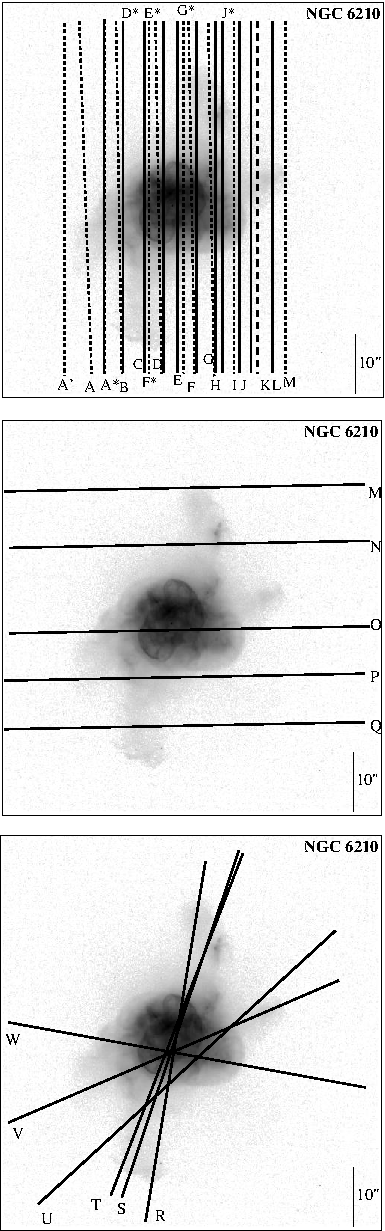
\includegraphics[width=0.4\textwidth]{tere-figs/Figure2a}
  \caption{Top panel shows the slit positions from the 2015 run, these are indicated as solid lines and 
labeled at the top against an [O III] HST image. Dashed lines refer to additional slit positions from other runs
and are labeled at the bottom of the image. The middle and bottom panels show the slit positions from 
the other runs placed at different position angles. }
  \label{fig:slit-positions}
\end{figure}



\begin{table}
\centering
\caption{OAN-SPM/Mezcal high-resolution spectroscopy of NGC~6210}
\label{table:pa5}
\begin{tabular}{l|cccccccc} \toprule
  &   Exp.~Time & Spectral  & Slit & P. A.   & slit        \\
  Epoch   &    (s) & Range  &  (\AA)    &    (\AA)  & (m$\mu$)     \\
  \midrule
1998/06/28          & 30 & \Ha  & 150 & 90 & O\\
1998/06/28          & 300 & \Ha  & 150 & 90 & N\\
1998/06/28           & 1200 & \Ha   & 150 & 90 & M,P,Q \\
2003/06/05         & 1800 &  \Ha   & 70 &0 &     A,B,D*,E*,F,H,I,K\\ 
2003/10/16   &  1800 &   \Ha    & 70 & $-$21 & T\\
2003/10/16    &  1800 &   \Ha   & 70 & $-$68 & V\\
2003/10/17    &  1800 &   \Ha  & 70 & 77 & W\\
2004/06/13   & 1800 &   \oiii  & 70 & $-$9 & R  \\  
2004/06/13   & 1800 &   \oiii  & 70 & $-$19 & S  \\  
2004/06/14    & 1800 &  \sii &150 & $-$19 & S  \\
2004/06/13   & 1800 &   \oiii  & 70 & $-$56 & U  \\  
2004/06/14   & 1800 &   \oiii  & 150 & 0 & A',L  \\
2011/05/21     & 1800 & \Ha  & 150 & 0 & G* \\
2011/05/21     & 600 & \oiii & 150 & 0  & G \\
2013/07/06    &  1800 & \Ha   & 150 & 0 & C,I,J \\
2015/08/18  &  1800 &   \Ha, \oiii  & 70 & 0 & C,D,E,F,G\\
2015/08/19  &  1800 &   \Ha, \oiii   & 70 & 0 & B,A*,I\\
2015/08/20   &  1800 &   \Ha, \oiii & 70 & 0 & H,J,K\\
2019/09/18  &  1800 &   \Ha    & 150 & 56 & \\
  \bottomrule
\end{tabular}
\end{table}

All data was reduced  by using standard IRAF\footnote{IRAF is
  distributed by the National Optical Astronomy Observatory, which is
  operated by the Association of Universities for Research in
  Astronomy, Inc. under cooperative agreement with the National
  Science foundation} routines. Bias and cosmic-ray removal was followed by rectification and first-order wavelength 
  calibration of the two-dimensional spectra based on the comparison
  the spectrum
of a Th/Ar lamp to an accuracy of $\pm$1 \kms{} when converted to
radial velocity.  All spectra presented in this paper are corrected to
heliocentric velocity (\vhel). 


The morphology of NGC 6210 varies significantly in high and low excitation images. In Figure 4 we show in the lower panels [O III] (left) and [N II] (right) archive $\rm HST$ images that clearly reveal the different structures from each ion.
The top panels are the corresponding images processed with a natural logarithm and edge detection algorithm where the most salient features are indicated and labeled for reference in the next sections.


Using FORTRAN and phython routines, we produced  velocity cubes in  \NIIlam{} and \oiii{} emission lines, in order to 
...

The resulting data cubes for the \Halam\, and \NIIlam\, lines are shown
in Figure 3 as isovelocity channel maps, each isovelocity map is 20
\kms\, wide. 


%\section{KINEMATICS}
%\label{sec:kinematic}

%The Figure 3 shows the \Halam{},  \OIIIlam{}, and \NIIlam{} velocity arrays, {\it P--V}, for all individual slit position, observed on 2015 epoch:   The stellar continuum from the central star
%has not been subtracted. . The expansion velocity of the inner shell, v$_{exp}$ = 28 \kms.





 % \caption{{\it Left:} Location of each slit position is indicated and
 %   labeled on an HST \OIIIlam, image of the NGC~6210. North is up,
 %   east left}

%\begin{figure*}
%\centering
%  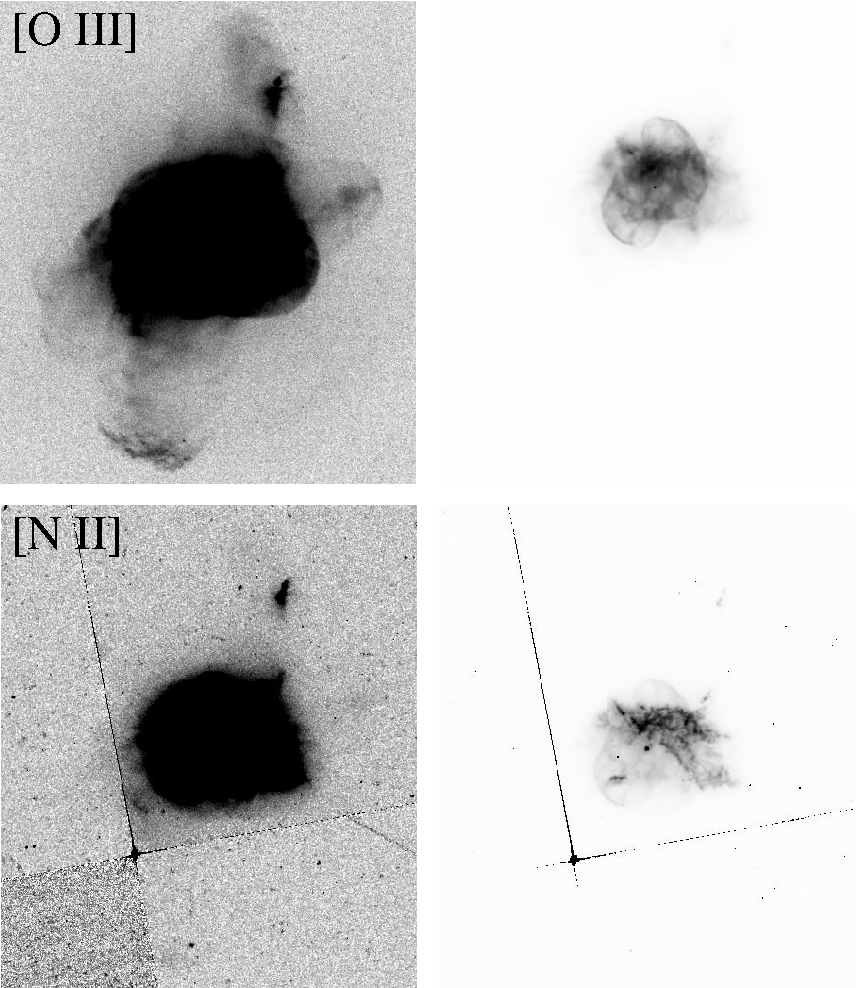
\includegraphics[width=0.7\textwidth]{tere-figs/Figure1}
%  \caption{ }
%\end{figure*}




\begin{figure*}
  \centering
  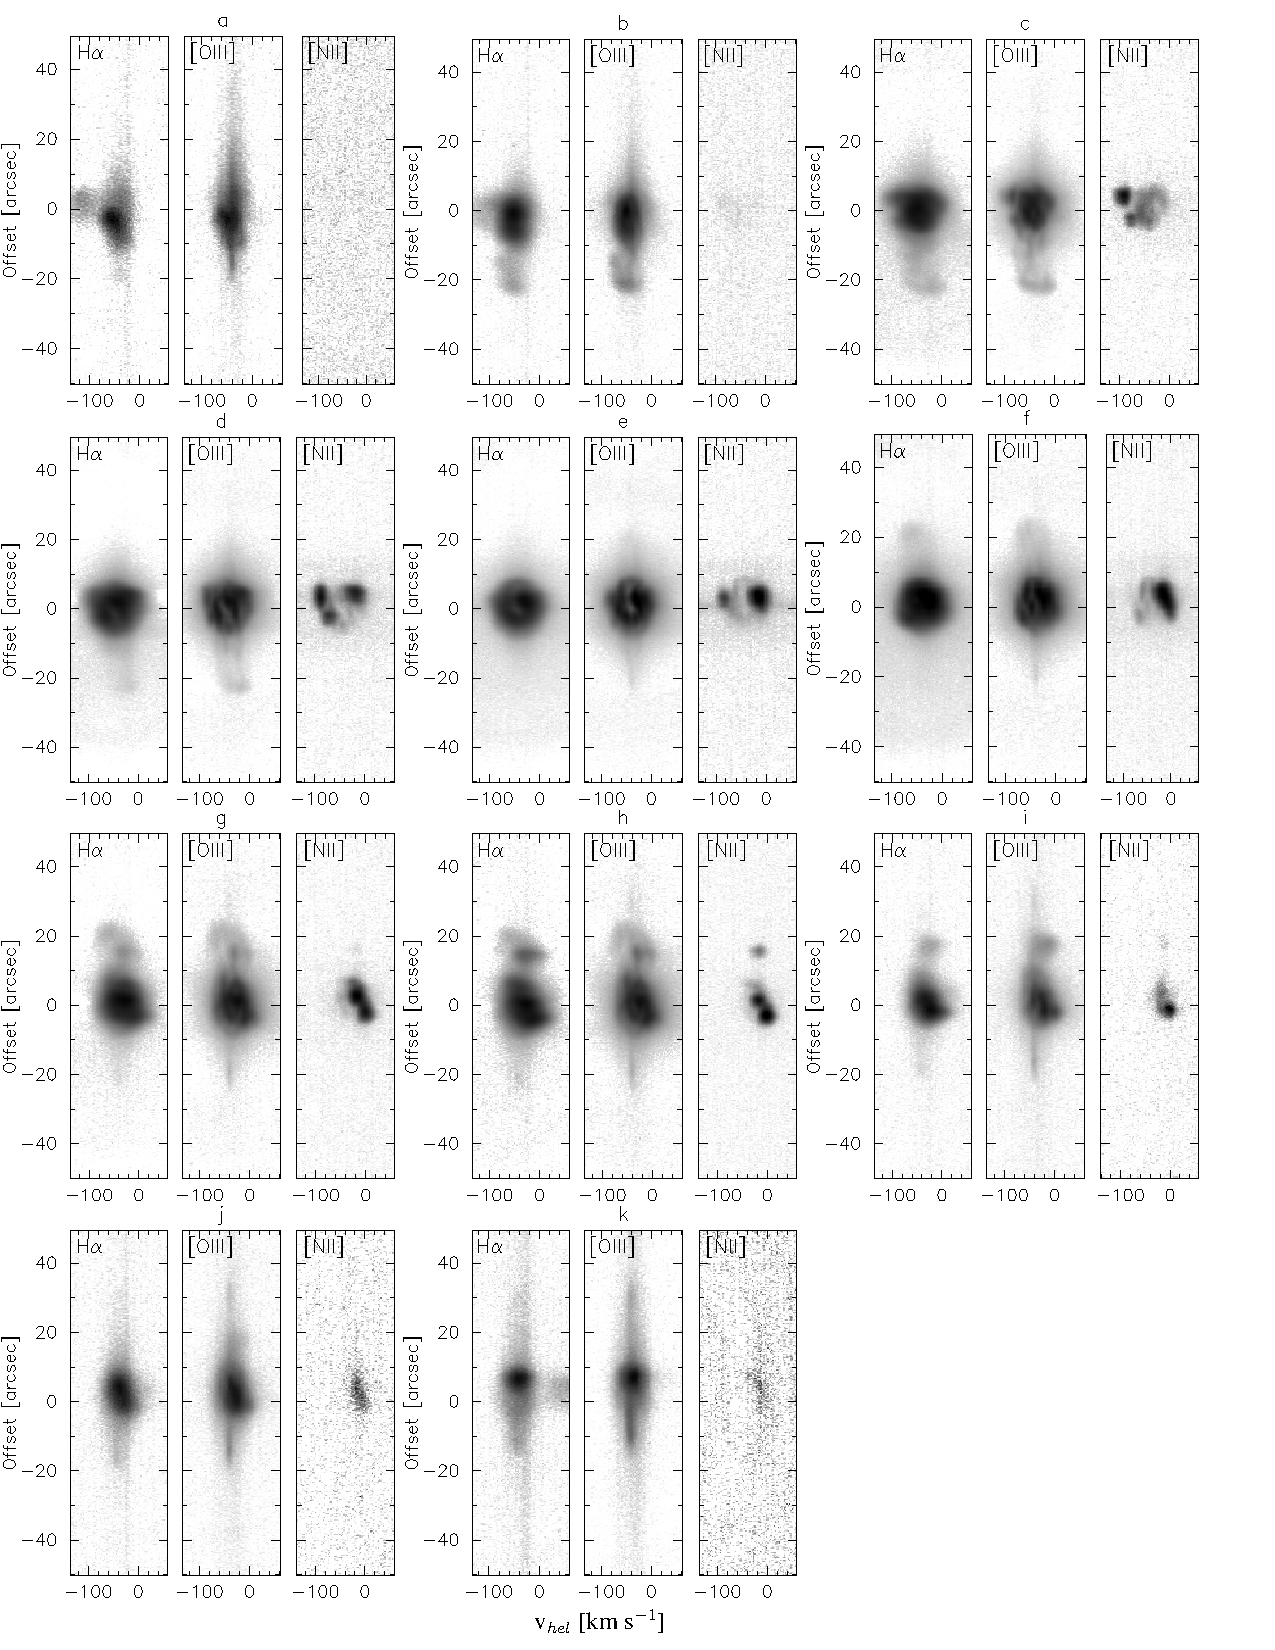
\includegraphics[width=1\textwidth]{tere-figs/Figure3}
  \caption{Position--velocity line profiles for the slit positions from the 2015 run are shown in sets where
the H$\alpha$ bi-dimensional line profile is on the left panel of the set, the \oiii{} line profile is on the central panel 
and the \nii{} line profile is on the right panel. The corresponding slit positions are indicated at the top of
each set of line profiles. The velocity scale is heliocentric and the spatial scale is indicated in arcsec 
with respect to the center of the nebula.}
  \label{fig:pv-array}
\end{figure*}




\begin{figure}
  \centering
  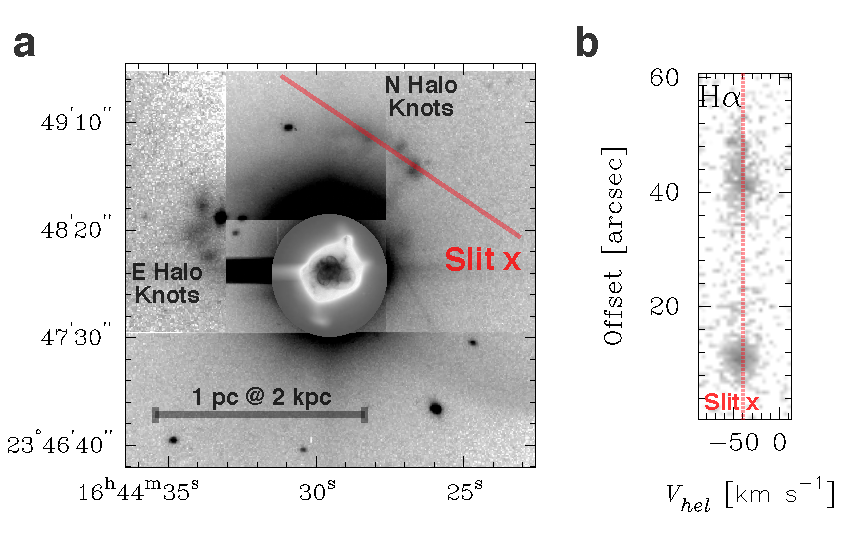
\includegraphics[width=\linewidth]{figs/turtle-halo-slit-x}
  \caption{
    Deep images and spectra of the outer halo of NGC~6210, showing knotty structure.
    (a)~Composite mosaic of \oiii{} images,
    each with an exposure time of 1800~s,
    giving a combined field of view of \(3' \times 3'\) centered on the nebula.
    The position of slit position X is shown, for which a deep \Ha{} spectrum was obtained.
    Note that different sections of the mosaic are shown with different brightness normalizations,
    leading to abrupt jumps at the boundaries. 
    (b)~\Ha{} spectrum from Slit~X, showing emission from two of the halo knots.
    The red dotted line shows the nebular systemic velocity.
  }
  \label{fig:halo-knots}
\end{figure}






\begin{figure}
\centering
%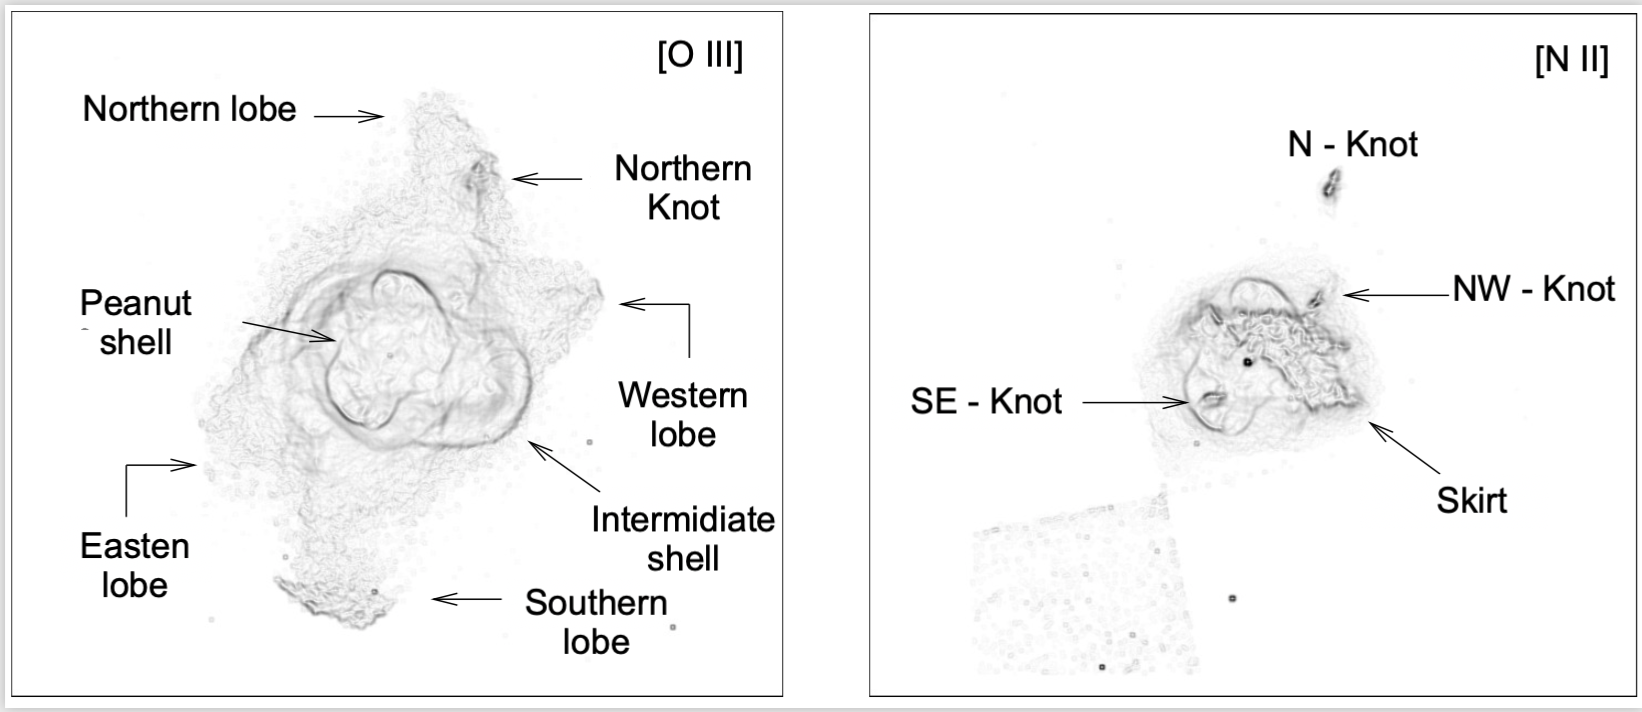
\includegraphics[width=0.7\textwidth]{tere-figs/Figure8}
%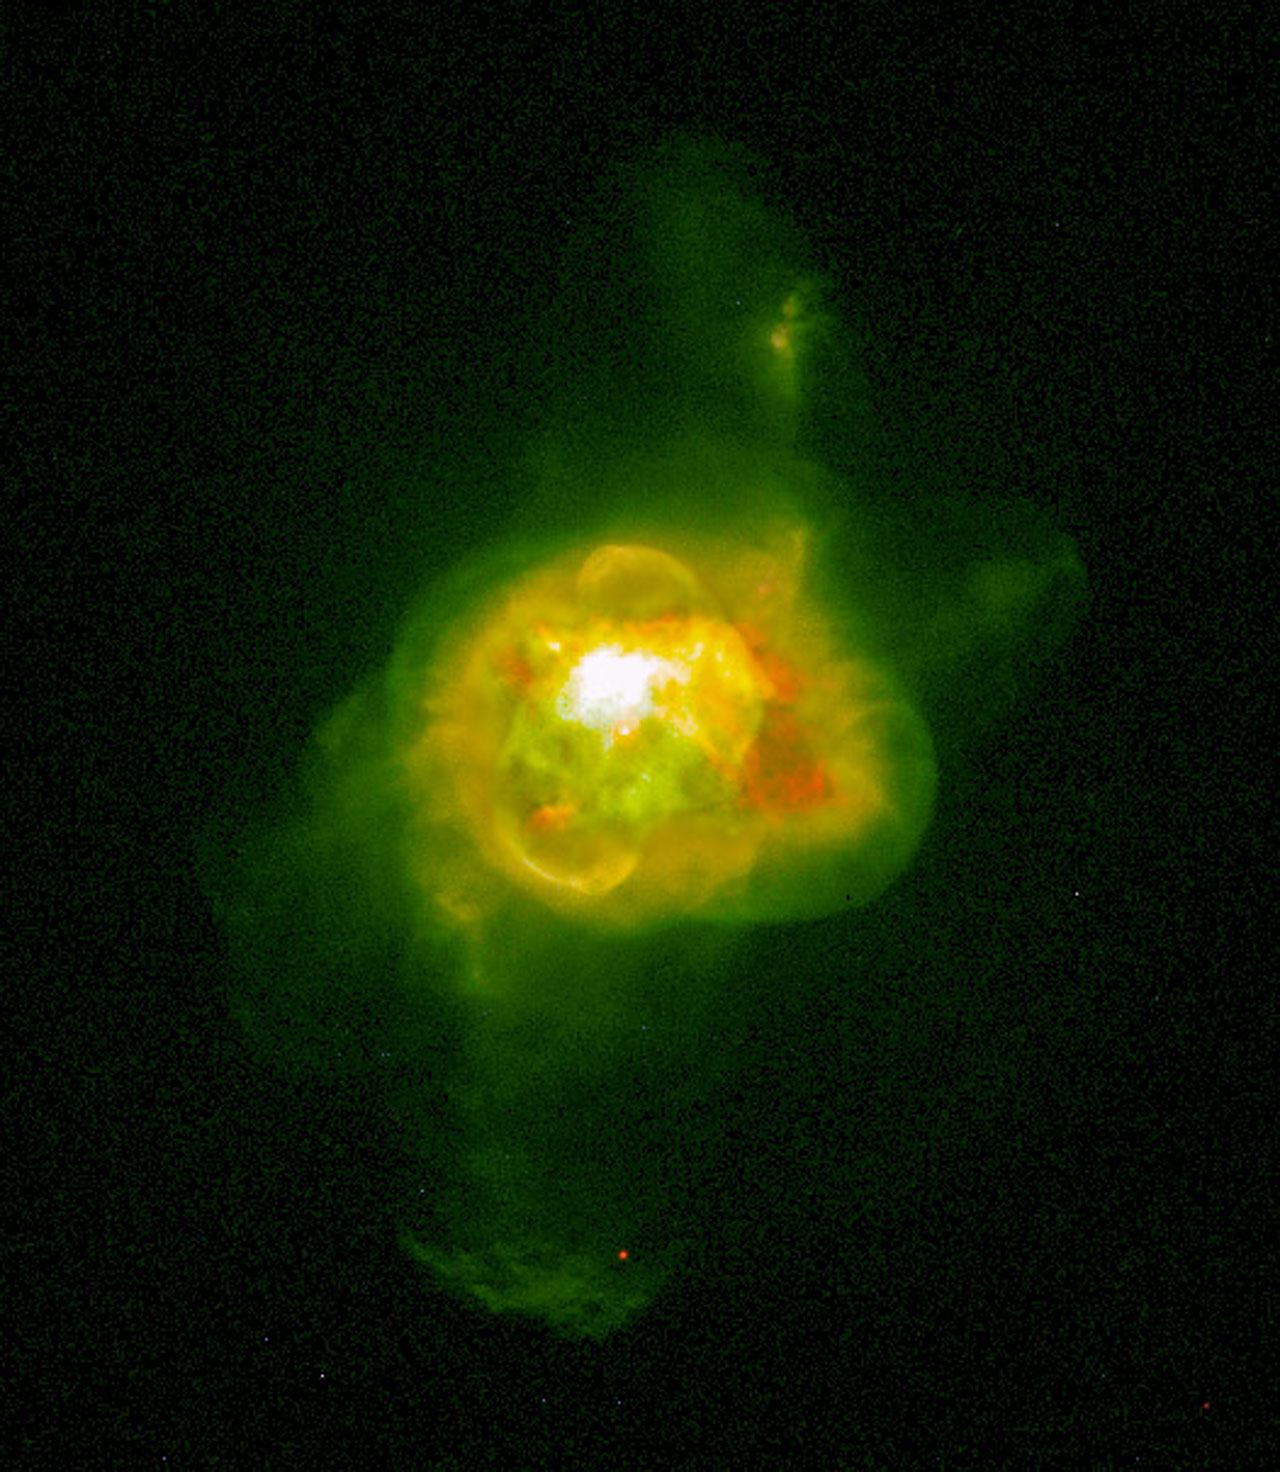
\includegraphics[width=0.327\textwidth]{tere-figs/opo9836f}
%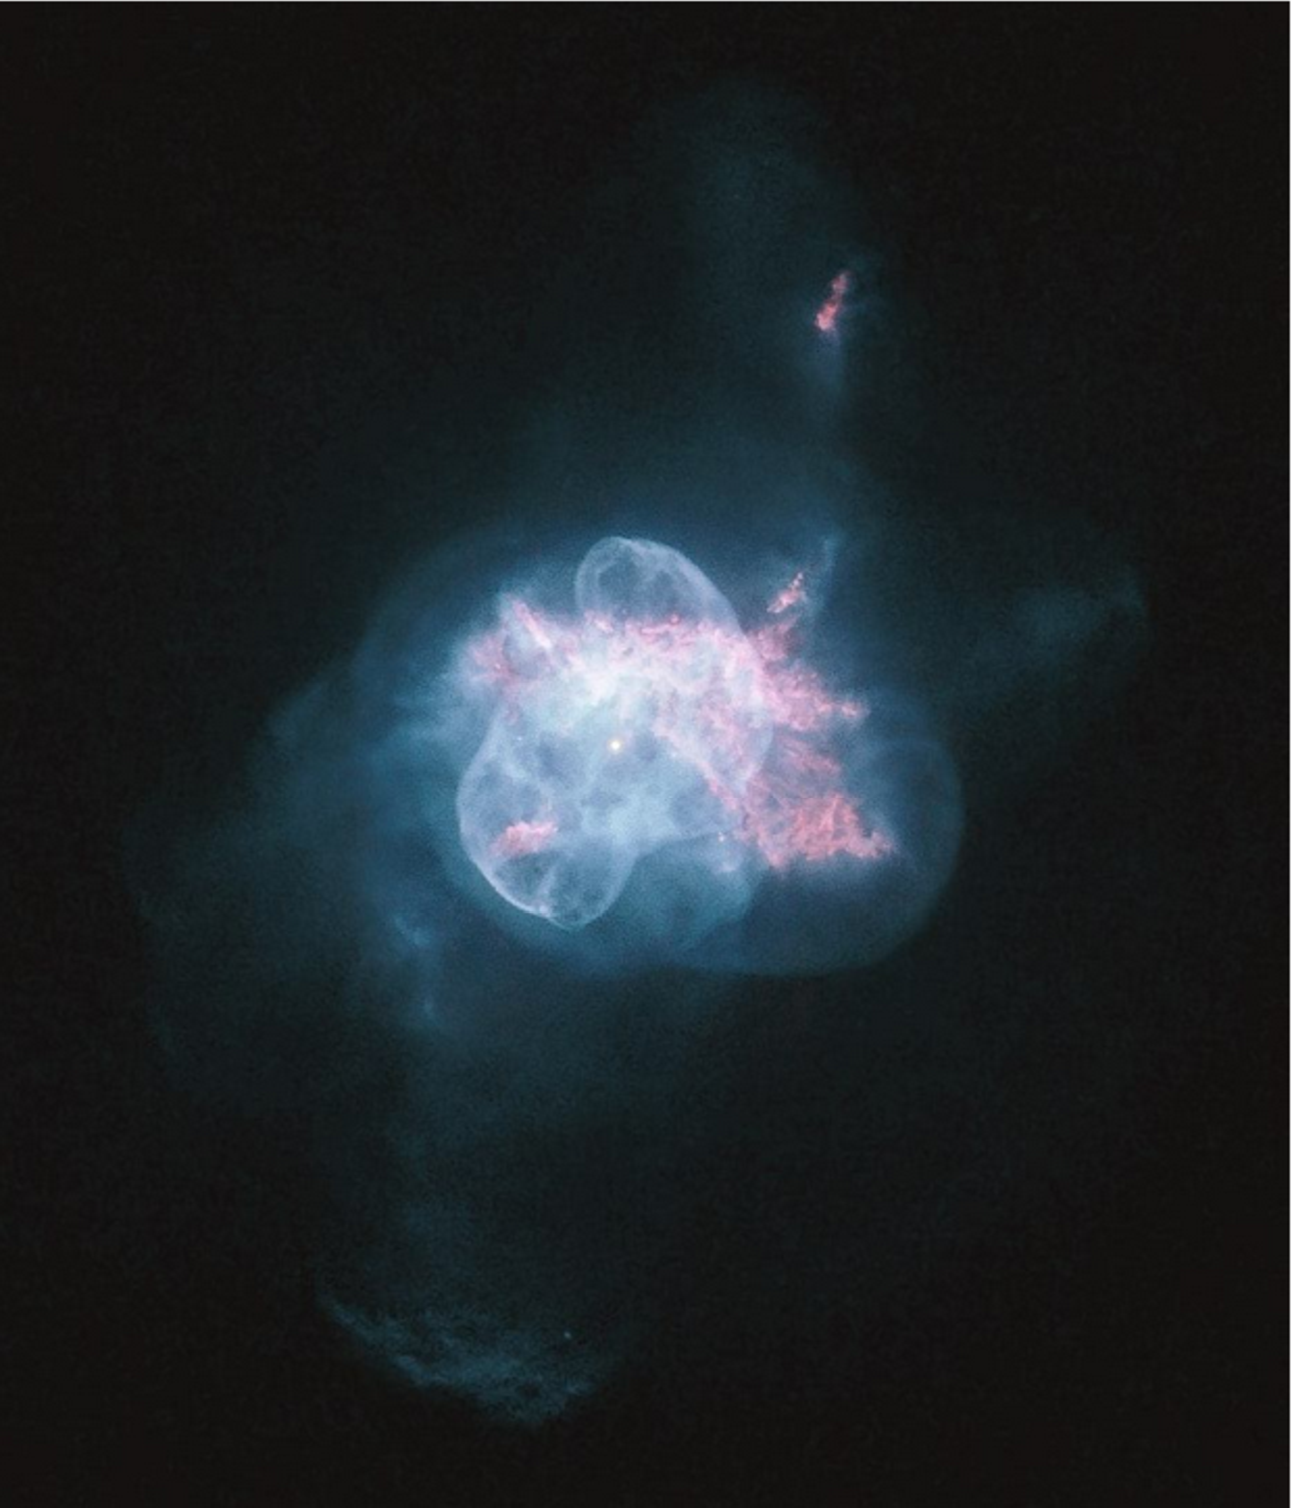
\includegraphics[width=0.32\textwidth]{tere-figs/N6210_ruso}
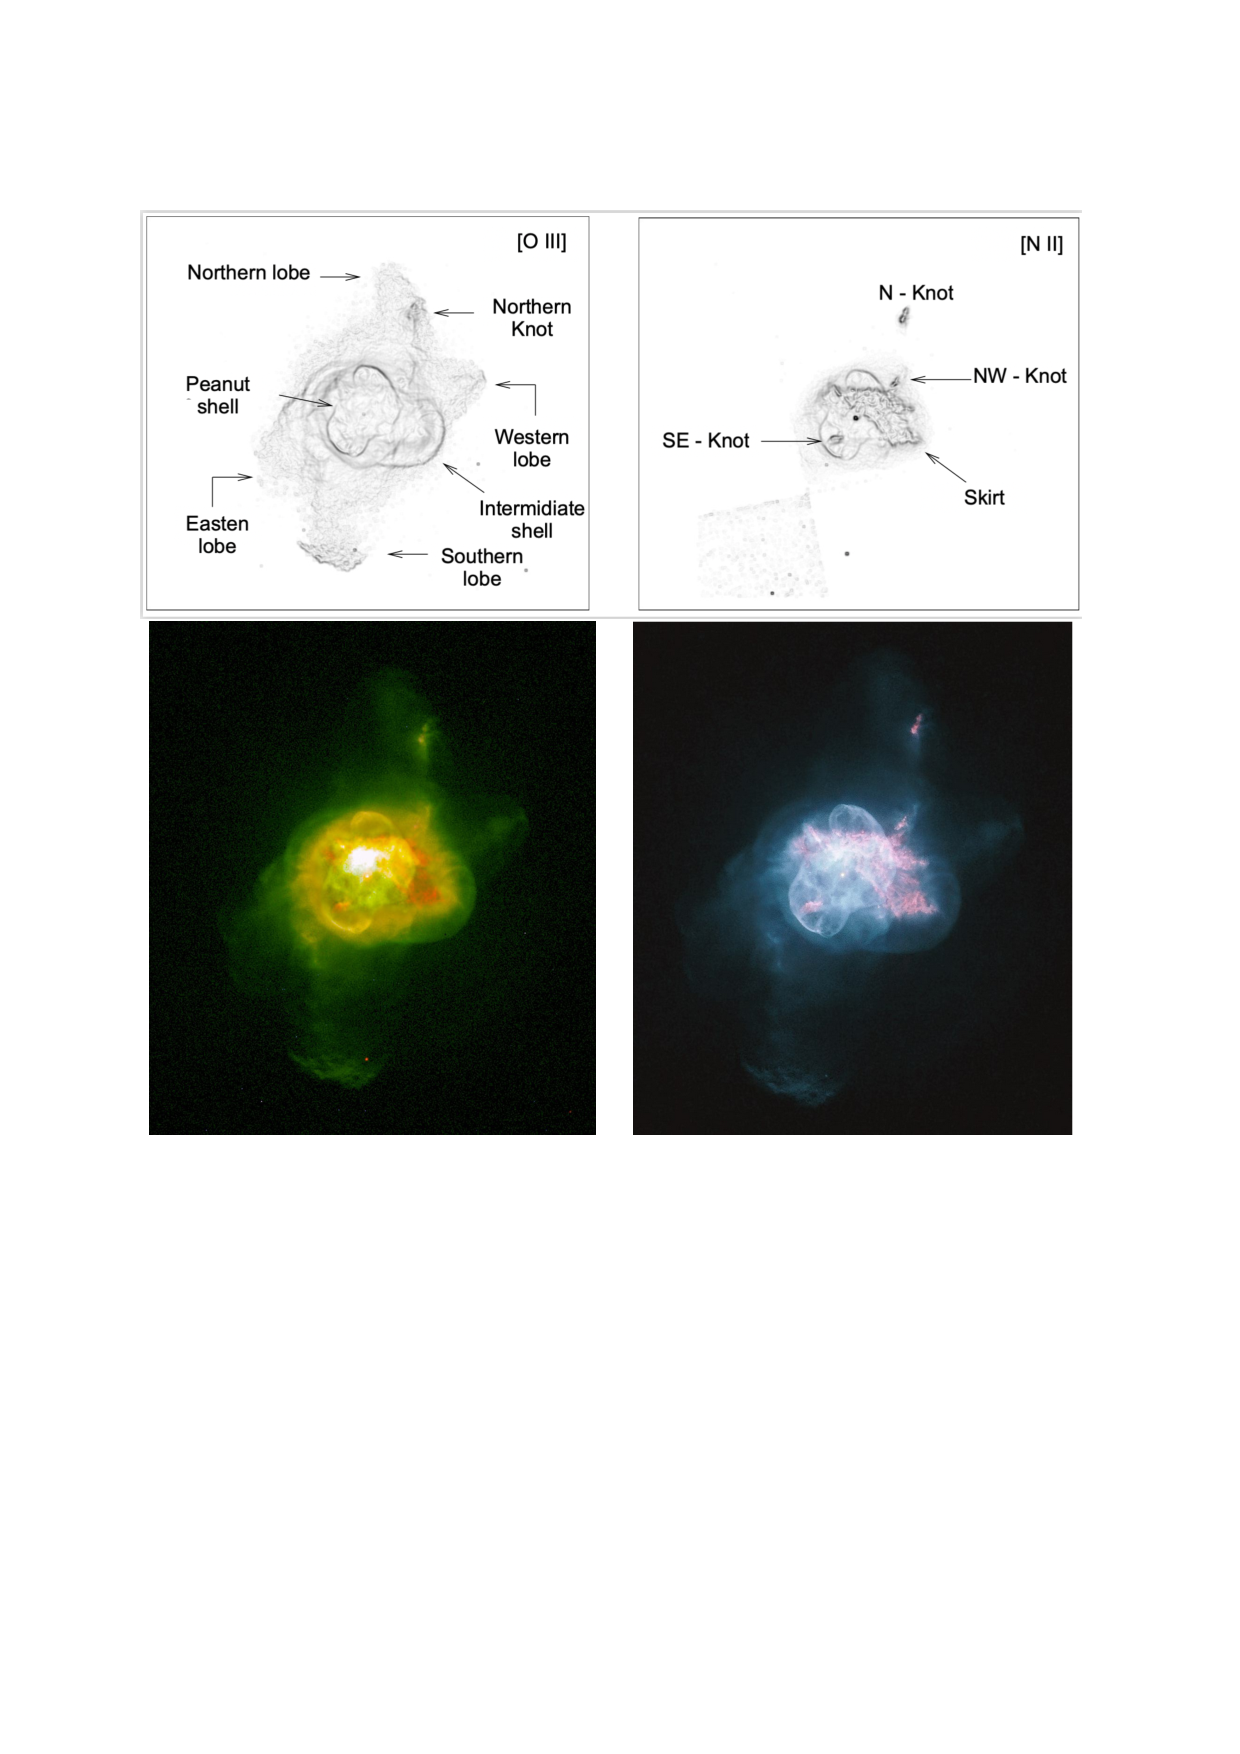
\includegraphics[width=\linewidth]{sketch}
\caption{mages from the HST archive are shown on the bottom panels,  \oiii{} (left) and \nii{} (right), and their
corresponding images are shown in the top panels processed with a natural logarithm function and an edge 
detection algorithm. The most salient features in these images are indicated and labeled for reference.}
\label{fig:hst}
\end{figure}








%\begin{figure*}
%\centering
%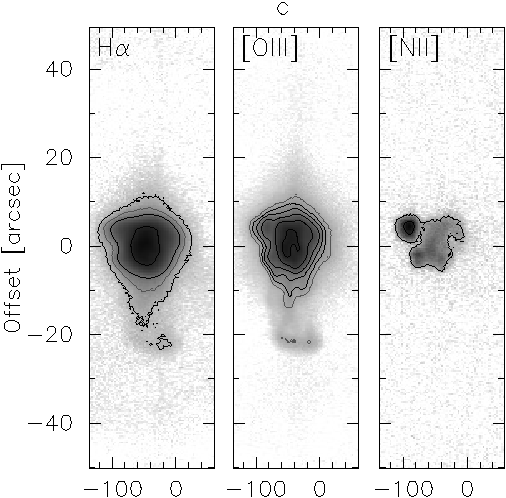
\includegraphics[width=0.9\textwidth]{tere-figs/rendija-c-cont}
%  \caption{  }
%\end{figure*}



%\begin{figure*}
%\centering

%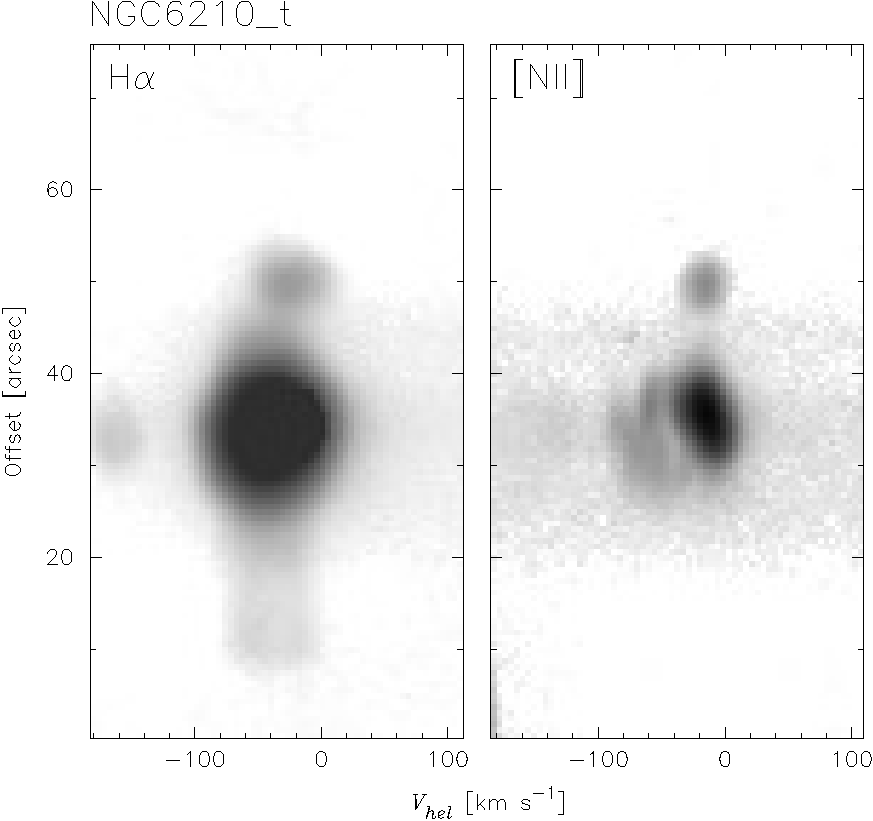
\includegraphics[width=0.4\textwidth]{tere-figs/slit_t_ha_nii}
%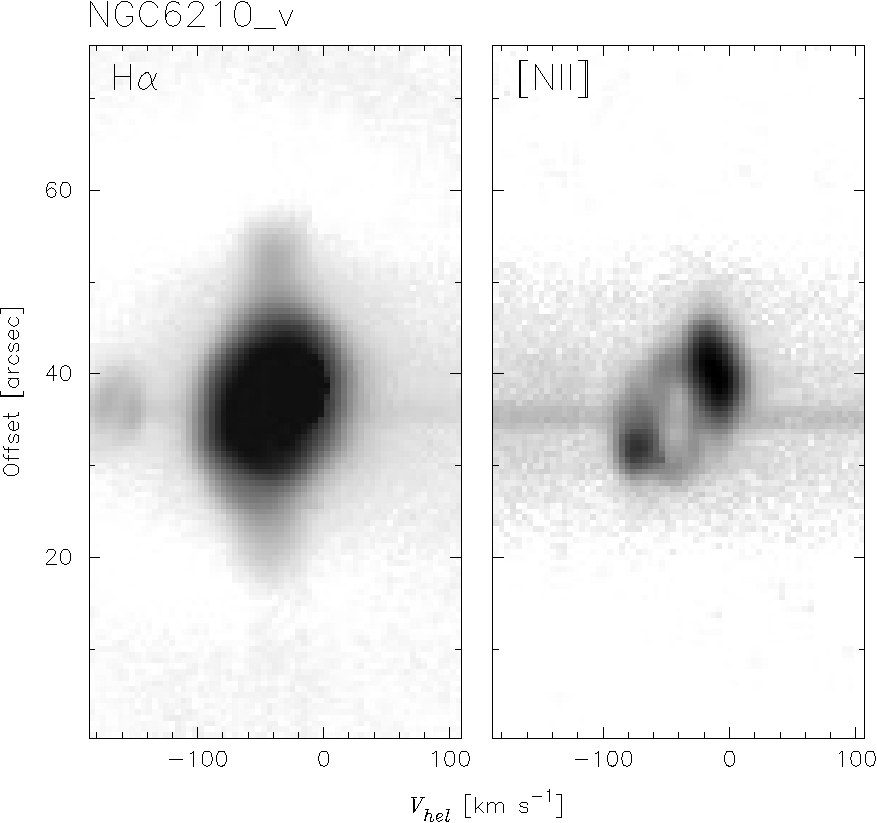
\includegraphics[width=0.4\textwidth]{tere-figs/slit_v_ha_nii}
%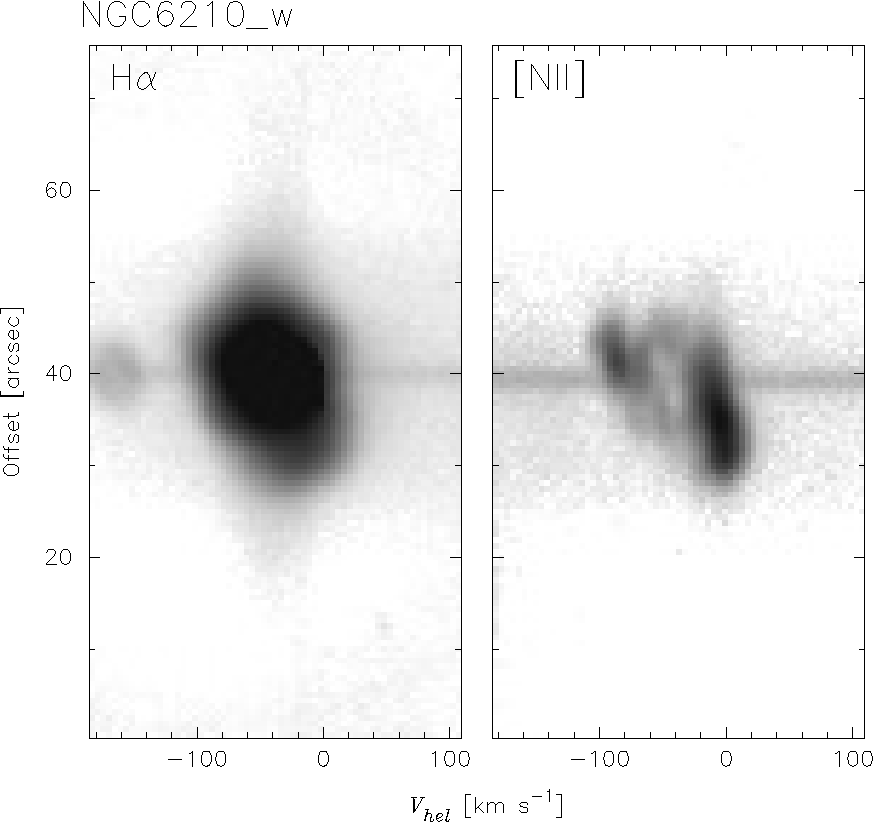
\includegraphics[width=0.4\textwidth]{tere-figs/slit_w_ha_nii}
%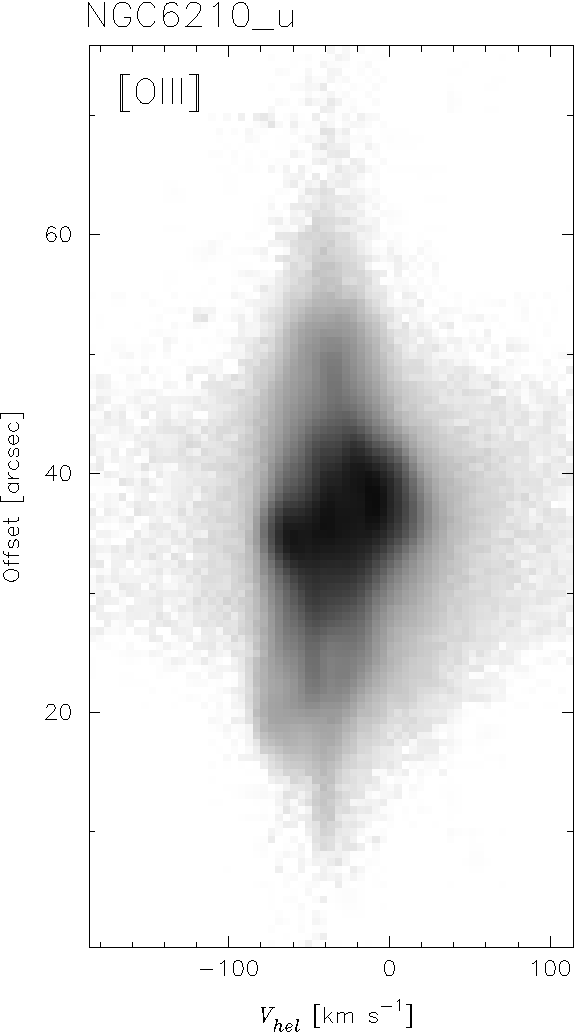
\includegraphics[width=0.2\textwidth]{tere-figs/slit_u_oiii}
%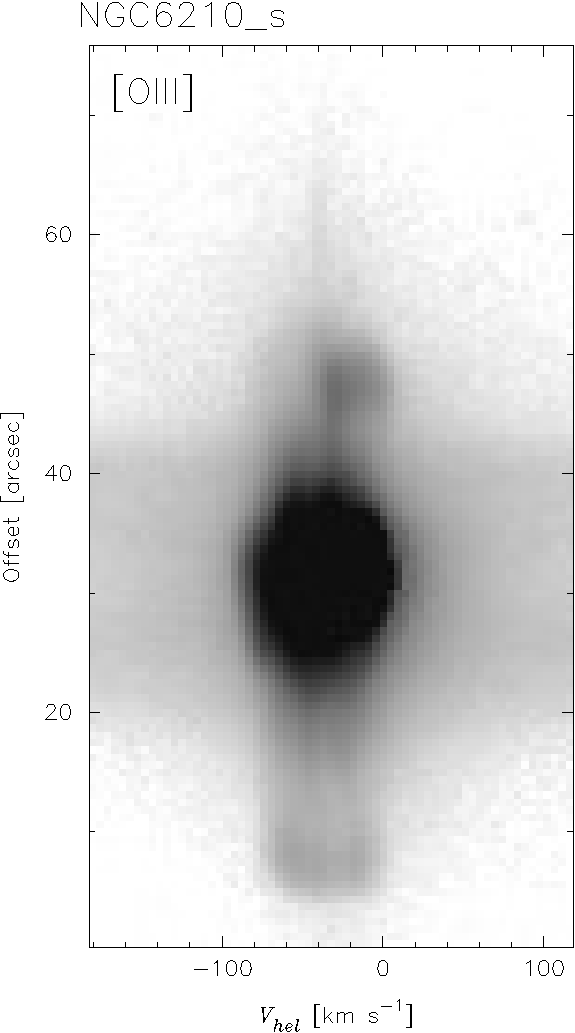
\includegraphics[width=0.2\textwidth]{tere-figs/slit_s_oiii}
%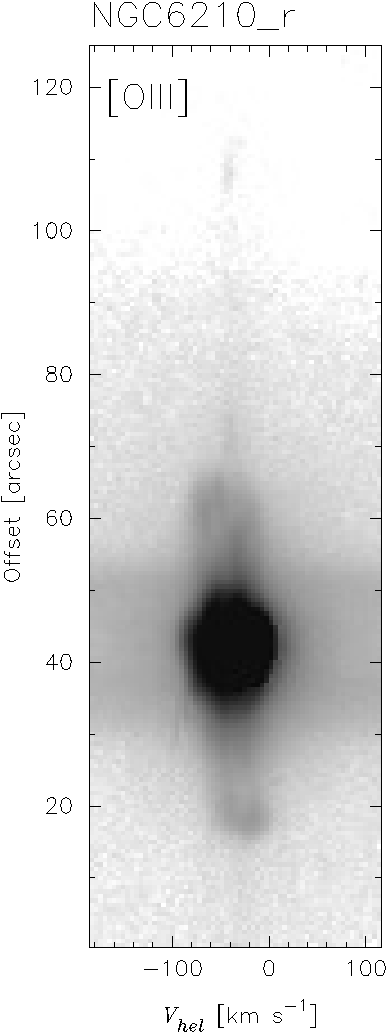
\includegraphics[width=0.2\textwidth]{tere-figs/slit_r_oiii}

  %\caption{  }
%\end{figure*}



\begin{figure}
  \centering
  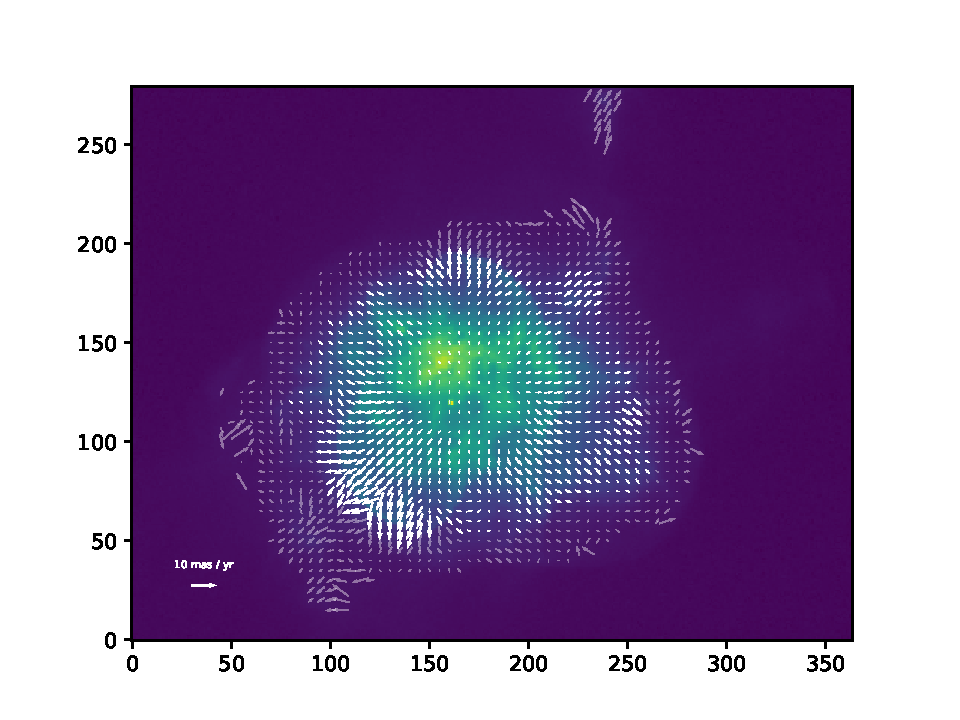
\includegraphics[width=\linewidth]{figs/oiii-propermotions}
  \caption{Proper motions derived from two HST \oiii{} images (F502N
    filter) separated by 10.45 years, using the FLCT algorithm with a
    Gaussian window width of 10~pixels. The key at bottom left shows a
    proper motion of \SI{10}{mas.yr^{-1}}, corresponding to
    \SI{95}{km.s^{-1}} for an assumed distance of \SI{2}{kpc}.}
  \label{fig:proper-motions-oiii}
\end{figure}
\begin{figure}
  \centering
  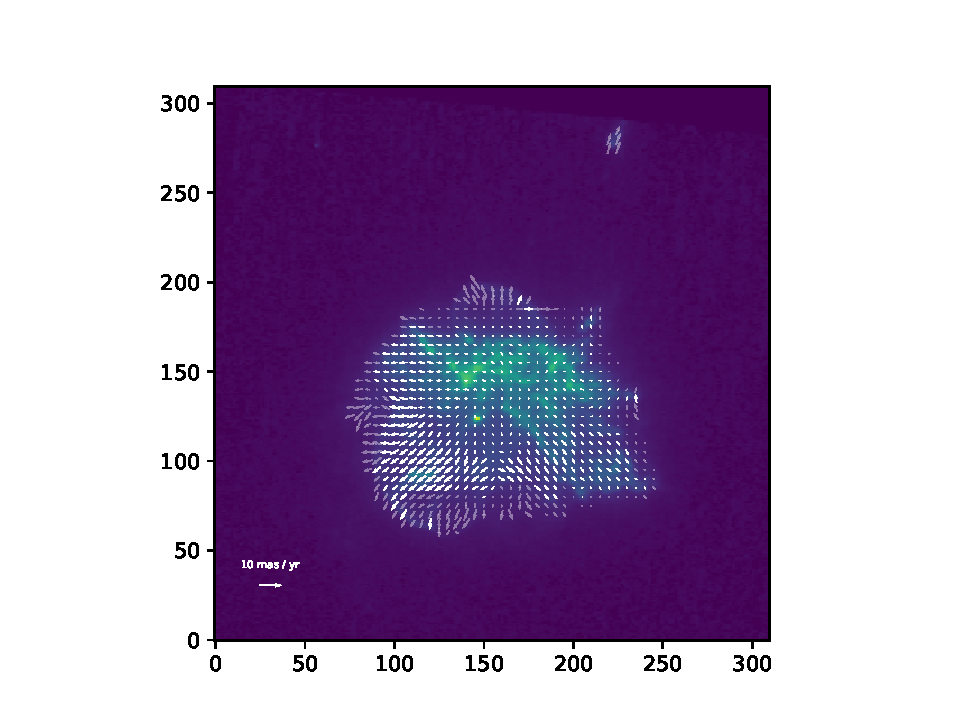
\includegraphics[width=\linewidth]{figs/nii-propermotions}
  \caption{As Fig.~\ref{fig:proper-motions-oiii} but for two HST
    \nii{} images (F658N filter). Note that the field of view is
    cropped slightly smaller than for \oiii{}.}
  \label{fig:proper-motions-nii}
\end{figure}

\begin{figure*}
  \centering
  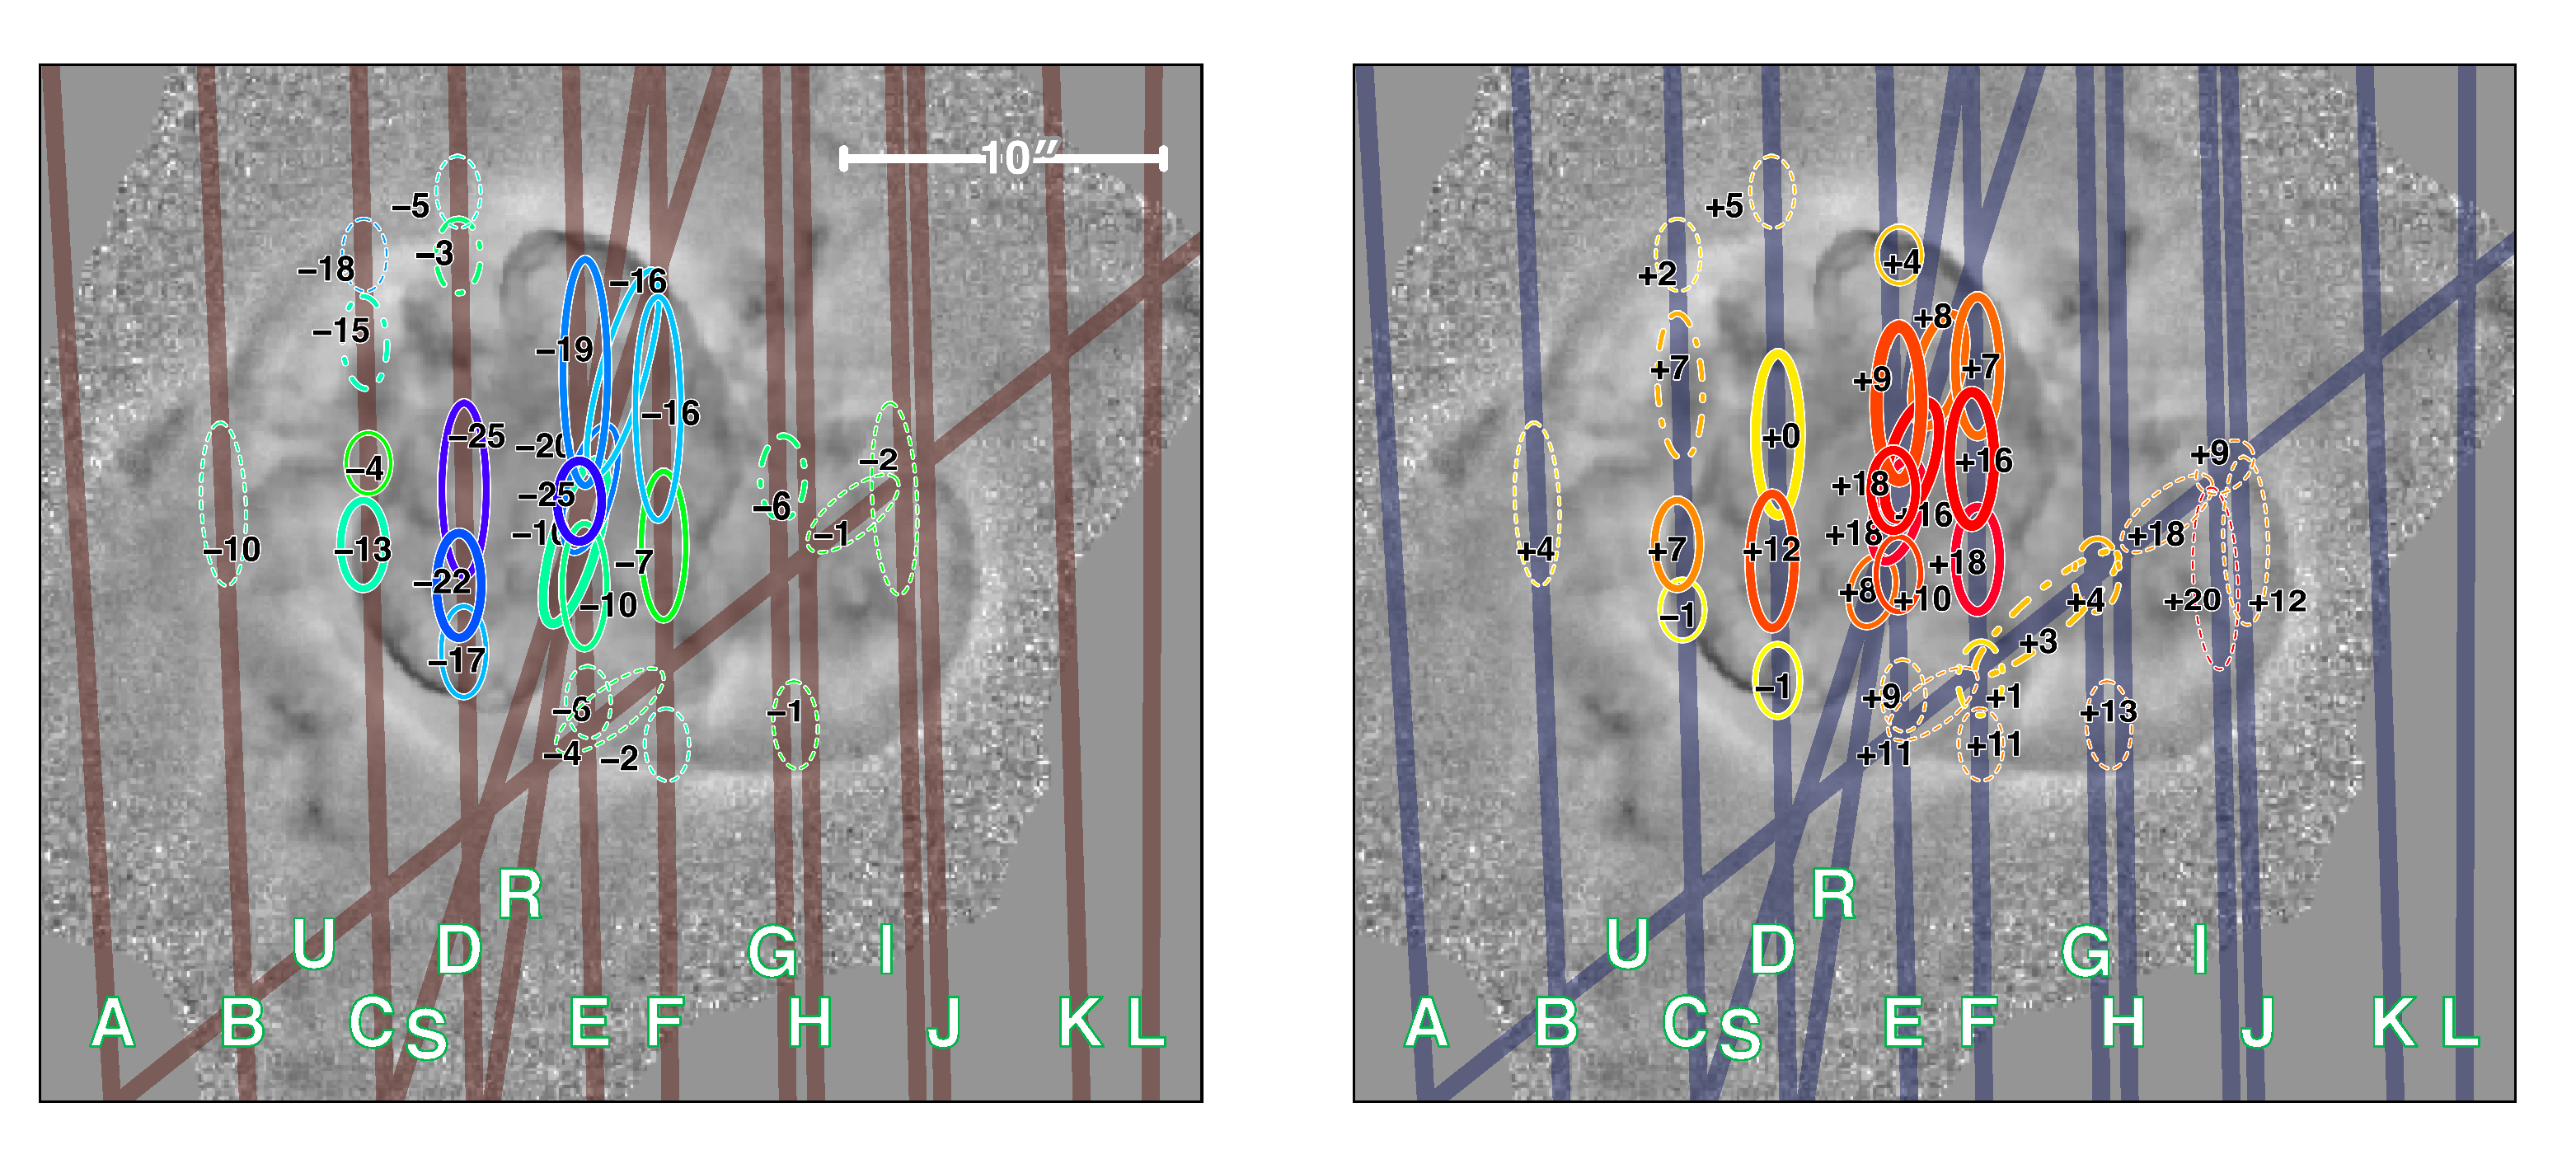
\includegraphics[width=\linewidth]{figs/turtle-peanut-map}
  \caption{
    Velocity features in the high-ionization shells,
    which have been identified in the \oiii{} slits.
    Left panel shows blue-shifted features,
    while right panel shows red-shifted features,
    each labelled with their line-of-sight velocity
    with respect to the nominal systemic velocity of \SI{40}{km.s^{-1}}.
    Solid lines show features in the inner shells,
    dashed lines show features in the intermediate shell,
    and dot-dashed lines show miscellaneous features between the two shells.
    The line width is a qualitative indicator of the brightness of each feature.
    The background grayscale shows a high-pass filtered version of the HST \oiii{} image.
  }
  \label{fig:shell-velocity-components}
\end{figure*}

\begin{figure}
  \centering
  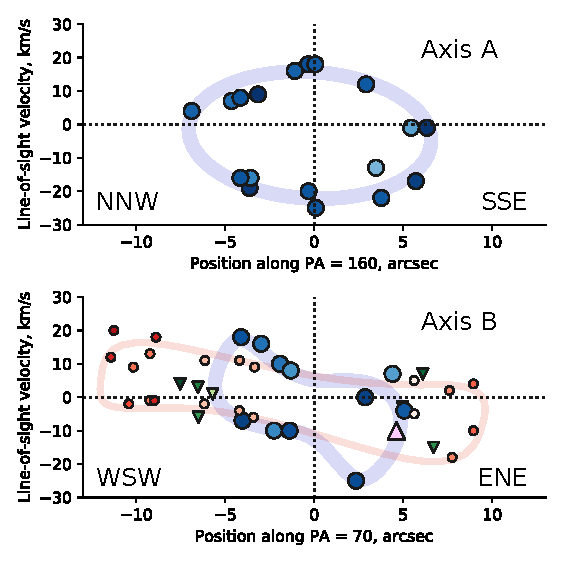
\includegraphics[width=\linewidth]{figs/turtle-shell-velocity-axes-annotated}
  \caption{
    Radial velocity versus position
    for the shell features shown in Fig.~\ref{fig:shell-velocity-components}.
    Results are shown along two axes:
    Axis~A (upper panel) is the apparent major projected axis of the inner shells,
    while Axis~B (lower panel) is perpendicular to this.
    Large blue circles show the inner shell,
    small red circles show the intermediate shell,
    and green triangles show miscellaneous features between the two shells.
    Darker colors indicate features that are closer to each respective axis.
    Colored lines are merely to guide the eye,
    and show possible interpretations of the shell kinematics along the two axes.
  }
  \label{fig:shell-velocity-axes}
\end{figure}


\section{Proper motions}
\label{sec:proper-motions}

The data used in this study to measure the proper motions of the turttle nebula consist of images which were retrieved from the HST archive. The \nii{} observations were made in two separate observing runs: on 1998 June 30, as part of program 7501, with Hajian, Arsen R., as PI. During this run, six images were obtained with the WFPC2, with an exposure time of 100 s (three images) y 40 s (three images) using the F658N filter. The second-epoch data were obtained on 2008 January 18, from the science program 11122, with Bruce Balick, as PI, who employed the same configuration as in program 7501 to acquire three images with the F658N filter, using 400 s exposure times for all of them. For all of the images, we used the drizzled images (processed with Astrodrizzle). 

Proper motions are calculated from HST WFPC2 imaging at two epochs separated by approximately 10 years,
using the FLCT method \citep{Welsch:2004a, Fisher:2008a}.\footnote{
  We used version 1.07 of FLCT, obtained from \url{http://cgem.ssl.berkeley.edu/cgi-bin/cgem/FLCT/home},
  together with version 1.04 of the Python wrapper pyflct,
  obtained from \url{https://github.com/PyDL/pyflct}.}
Results are shown in Figures~\ref{fig:proper-motions-oiii} and~\ref{fig:proper-motions-nii} for \oiii{} and \nii{}, respectively.
In both cases, the images were remapped to a uniform square pixel grid at the WFC resolution of \SI{0.1}{arcsec.pix^{-1}} before applying the algorithm.
The resultant per-pixel motions between the two epochs are found to be of order \SI{0.5}{pix} (\(\approx \SI{5}{mas.yr^{-1}}\))
and these raw results were then corrected by applying a global shift to force the motion of the central star to be zero.
The systematic error from the global alignment of the two epochs is estimated to be \SI{1.5}{mas.yr^{-1}},
which is expected to dominate the proper motion uncertainties in the brighter parts of the nebula.
In fainter and more featureless regions of the nebula, the proper motions are increasingly affected by random noise,
which can be seen in parts of the lobes in Figure~\ref{fig:proper-motions-oiii}.

The corrected results, as shown in the figures, can be seen to display motions that are predominantly radial from the central star.
To convert the angular motions into transverse velocities, we assume a distance of \SI{2}{kpc},
so that \SI{10}{mas.yr^{-1}} is equivalent to \SI{95}{km.s^{-1}}.
From the \oiii{} images (Fig.~\ref{fig:proper-motions-oiii}),
the fastest plane-of-sky motions are of order \SI{60}{km.s^{-1}},
and are chiefly along the NNW--SSE direction,
including the projected major axis of the inner peanut shell,
the NW~knot, the N~jet, and the end-cap of the S~lobe.
Motions along the perpendicular ENE--WSW direction are typically slower,
of order \SI{30}{km.s^{-1}}.
Note that proper motions are unavailable for the end cap of the N lobe since the second epoch HST image does not cover this region.

The \nii{} images (Fig.~\ref{fig:proper-motions-nii}) show a similar expansion pattern for the features that are visible in both lines.
Remarkably low plane-of-sky velocities of \(\le \SI{15}{km.s^{-1}}\) are seen for the \nii{}-bright knot complexes immediately north and west of the central star. 

Previously, \citet{Schonberner:2018a} have also studied the proper motions
in the Turtle Nebula, based on the same HST observations as those used here.
They employ a magnification method, which implicitly assumes a homologous expansion,
finding a magnification factor over the 10 to 11-year baseline
of \(M = 1.0085 \pm 0.0005\) for the inner high-ionization shells
(which they call the cavity rim)
and \(M = 1.0055 \pm 0.0005\) for the low-ionization knot complexes (see their Table~2).
After conversion to velocity units (assuming a distance of \SI{2}{kpc}),
these are consistent within the stated errors with our own average results for each of these two nebular components.

\section{Kinematic components from slit spectra}
\label{sec:kinematic-components}

In order to investigate the kinematics of the nebula in detail,
we have measured the velocities of distinct emission components in each slit spectrum
and organized them into broad systems based on their location, morphology and degree of ionization.

\subsection{High-ionization shells}
\label{sec:high-ioniz-shells}

These systems represent the majority of the \oiii{} emission in the core of the nebula
and show a nested elliptical shell morphology.
Figure~\ref{fig:shell-velocity-components} shows the \oiii{} emission components associated with these shells,
as derived from the longslit spectra.
Line-of-sight velocities are given with respect to the nominal systemic velocity (\SI{40}{km.s^{-1}} heliocentric),
separated into negative velocities (left panel) and positive velocities (right panel).
The inner ``peanut'' shells, with a radius of \(5''\) to \(7''\), are the brightest
and are indicated by thick-lined colored ellipses. 
The edge of the more extended intermediate shell, with a radius of \(8''\) to \(12''\), is 10 to 100 times fainter than the inner shells
and is indicated by thinner dashed ellipses.
Additional miscellaneous emission features located in between these shells are indicated by dot-dashed ellipses.
Further features that seem to be associated with the low-ionization knots discussed below in \S~\ref{sec:knot-complexes} are omitted from the figure.


Although the inner shell is irregular in shape,
it shows an apparent elongation along \(\text{PA} \approx \ang{160}\).
The intermediate shell is elongated roughly perpendicular to this, along \(\text{PA} \approx \ang{70}\).
In Figure~\ref{fig:shell-velocity-axes} we plot the velocity of each shell component
against position along each of these axes,
which we denote axis~A and axis~B.  
Each component was assigned to only one axis (A or B), according to its location,
but this assignment is unavoidably subjective for components near the center,
where the two axes cross.

Along axis~A a closed velocity ellipse can be seen for the inner shells,
with a maximum splitting of \(\pm \SI{22}{km.s^{-1}}\) close to the central star
and velocities close to zero at either end (\(\pm 7''\)).
The pattern is not entirely symmetric,
with a slight gradient of \(\pm \SI{3}{km.s^{-1}}\) along the length,
in which the more negative velocities are at the SSE end.
The centroid of the ellipse is also shifted by \(\SI{-3.5}{km.s^{-1}}\)
with respect to the systemic velocity.

Along axis~B,
which is the apparent minor axis of the inner shells (\(\pm 5''\)),
the ellipse is distorted and the gradient is much more pronounced:
\(\pm \SI{11}{km.s^{-1}}\),
with the more negative velocities at the ENE end
(large blue circle symbols in lower panel of Fig.~\ref{fig:shell-velocity-axes}).
Velocity splitting of \(\pm \SI{9}{km.s^{-1}}\) is seen near both ends,
but it is not clear from the \oiii{} spectra if the ends are closed or open,
since none of the \oiii{} slits are aligned with this axis.
However, one of the \nii{} slits (slit~W) is indeed oriented close to axis~B and,
although the shells emit only weakly in \nii{},
the distorted ellipse is clearly closed at the ENE end
(large pink triangle symbol in Fig.~\ref{fig:shell-velocity-axes}).
The situation is not so clear at the WSW end
since any \nii{} emission from the shell is swamped by brighter emission from the knot complexes.
However, the evidence from \textit{HST} imaging suggests that the shell is closed in this direction also.

The intermediate shell along axis~B repeats a similar kinematic pattern to the inner shell,
but at larger radii.
It is represented by dashed ellipses in Figure~\ref{fig:shell-velocity-components} and small red circle symbols in Figure~\ref{fig:shell-velocity-axes}.
The gradient (\(\pm \SI{9}{km.s^{-1}}\)) and splitting (\(\pm \SI{8}{km.s^{-1}}\))
are both marginally smaller than for the inner shell.
Note that, unlike the inner shells, the intermediate shell is markedly lop-sided,
extending \(12''\) to the WSW, but only \(10''\) to the ENE.

The miscellaneous high-ionization components lie outside the inner shells
and show a spoke-like morphology on the \textit{HST} images.
They are represented by dot-dashed ellipses in Figure~\ref{fig:shell-velocity-components} and small green triangle symbols in Figure~\ref{fig:shell-velocity-axes}.
They do not show any marked kinematic pattern,
but are broadly compatible with the velocities of nearby portions of the intermediate shell. 


\begin{figure}
  \centering
  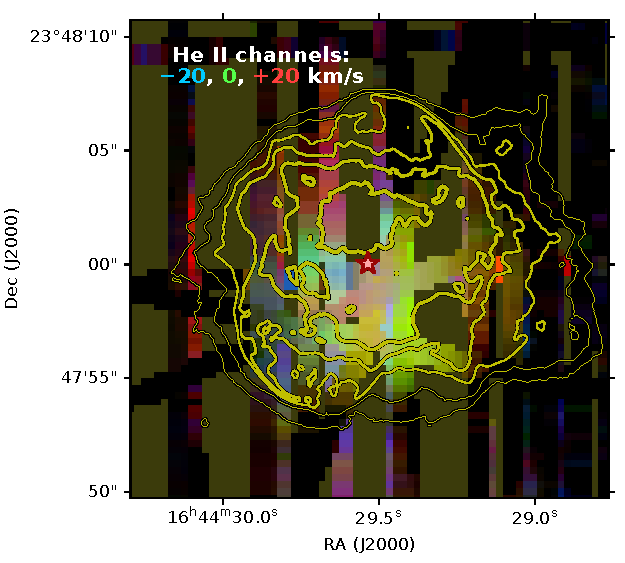
\includegraphics[width=\linewidth]{figs/turtle-heii-shell-annotated}
  \caption{
    Reconstructed velocity channel maps from the \heii{} slit spectra,
    showing the highest ionization gas in the nebula.
    The color image is constructed from 3 channels, each of width \SI{20}{km.s^{-1}},
    as indicated in the figure.  Contours show the \oiii{} HST image. 
  }
  \label{fig:heii-shell-annotated}
\end{figure}

\begin{figure*}
  \centering
  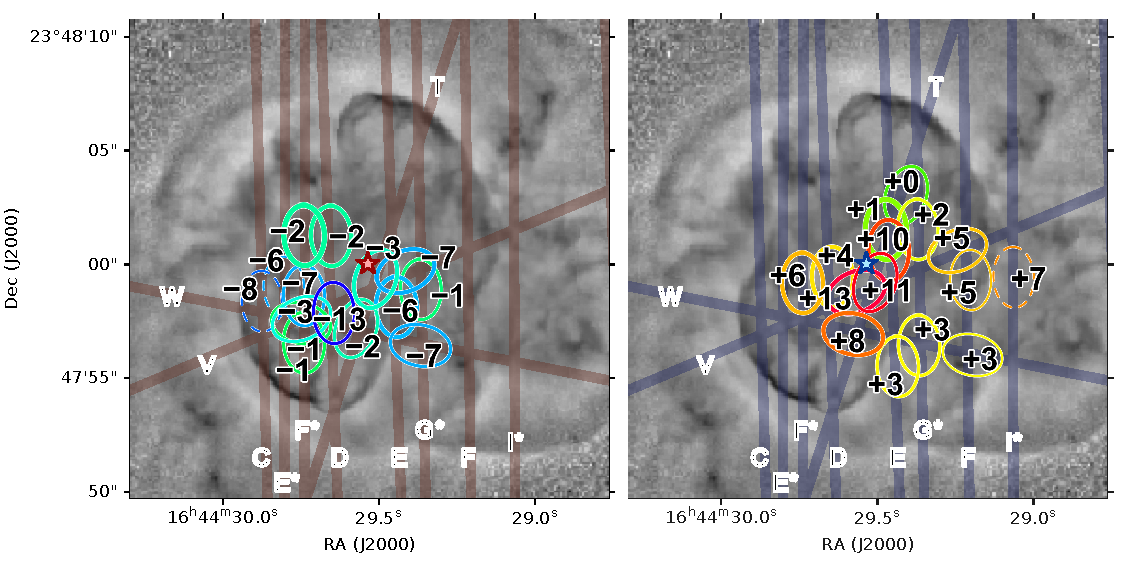
\includegraphics[width=\linewidth]{figs/turtle-heii-shell-components}
  \caption{
    Velocity features in the highest-ionization gas,
    which have been identified in the \heii{} slits.
    Left panel shows blue-shifted features,
    while right panel shows red-shifted features,
    each labelled with their line-of-sight velocity
    with respect to the nominal systemic velocity of \SI{40}{km.s^{-1}}.
    The line width is a qualitative indicator of the brightness of each feature,
    with dashed lines showing the very faintest features.
    The background grayscale image is the same as in Fig.~\ref{fig:shell-velocity-components}.
  }
  \label{fig:heii-shell-components}
\end{figure*}

\begin{figure}
  \centering
  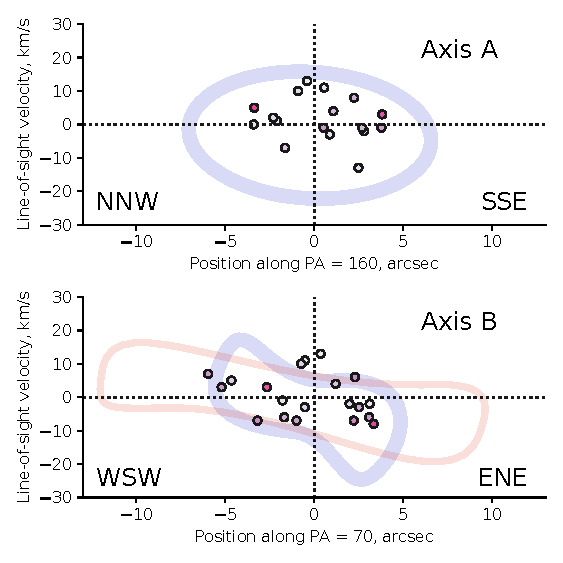
\includegraphics[width=\linewidth]{figs/turtle-heii-shell-velocity-axes-annotated}
  \caption{
    Radial velocity versus position
    for the \heii{} shell features shown in Fig.~\ref{fig:heii-shell-components}.
    Results are shown projected along along the same two axes
    as in Fig.~\ref{fig:shell-velocity-axes}:
    Axis~A (upper panel) and Axis~B (lower panel).
    Colored lines show the \oiii{} shells from Fig.~\ref{fig:shell-velocity-axes}.  
  }
  \label{fig:heii-shell-velocity-axes}
\end{figure}

In order to trace the more highly photo-ionized gas in the nebula,
we also analyze the weak \heii{} \SI{6560.10} line,
which is seen in the blue wing of the \Ha{} line,
displaced in velocity units by \SI{-123}{km.s^{-1}}.
Figure~\ref{fig:heii-shell-annotated} shows a three-color combination of channel maps in this line, reconstructed from our slit spectra.
It can be seen that the emission is more centrally concentrated than other emission lines
(contours show the HST \oiii{} image for comparison)
and is mainly confined to the inner peanut shells.
Note that the red channel is partially contaminated by \Ha{} emission in some slits.
It is also notable that the \heii{} emission is lop-sided in the opposite sense to the other emission lines,
with a brightness peak that is displaced \(\approx 2.5''\) to the south of the central star.
All three of the lines \Ha{}, \nii{}, and \oiii{} have a brightness peak that is displaced \(\approx 2''\) to the north of the central star.

Further details of the \heii{} kinematics are illustrated in Figure~\ref{fig:heii-shell-components},
which shows velocity features identified in the slit spectra.
For the slits that pass closest to the central star,
a full velocity ellipse is visible in the spectrum,
in which case four velocity components are measured,
two corresponding to the maximum spatial extension
and two to the maximum velocity splitting.
For other slits, only a partial ellipse is seen and fewer velocity components are measured.
As expected for an expanding shell structure, the largest absolute velocities (blue and red)
are seen close to the center,
with smaller absolute values around the periphery.
On the other hand, there is also a clear tendency for bluer velocities towards the east
and redder velocities towards the west.

Figure~14 shows the \heii{} velocity components projected on to the same two axes,
A and B,
which were found above from analysis of the \oiii{} shell kinematics.
The velocity and spatial scales are the same as in Figure~\ref{fig:shell-velocity-axes}
and the approximate loci of the \oiii{} shells are indicated by solid lines,
which allows the \oiii{} and \heii{} kinematics to be easily compared.
The maximum \heii{} velocity splitting of \(\pm \SI{13}{km.s^{-1}}\) is a little more than half as large as is seen in \oiii.
Along axis~A, the \heii{} emission is also more spatially compact than in \oiii{}.
Along axis~B, on the other hand, the \heii{} emission has a similar spatial extent to the inner \oiii{} shell,
even extending slightly beyond the inner shell on the WSW side
(for instance, the \heii{} component detected in slit~I\(^*\), as shown in the right panel of Fig.~\ref{fig:heii-shell-components}).
A gradient of \(\pm \SI{7.5}{km.s^{-1}}\) is seen along axis~B,
which has the same sense as the slightly larger gradient seen in \oiii{} along the same axis.

\subsection{Low-ionization knot complexes}
\label{sec:knot-complexes}

\begin{figure*}
  \centering
  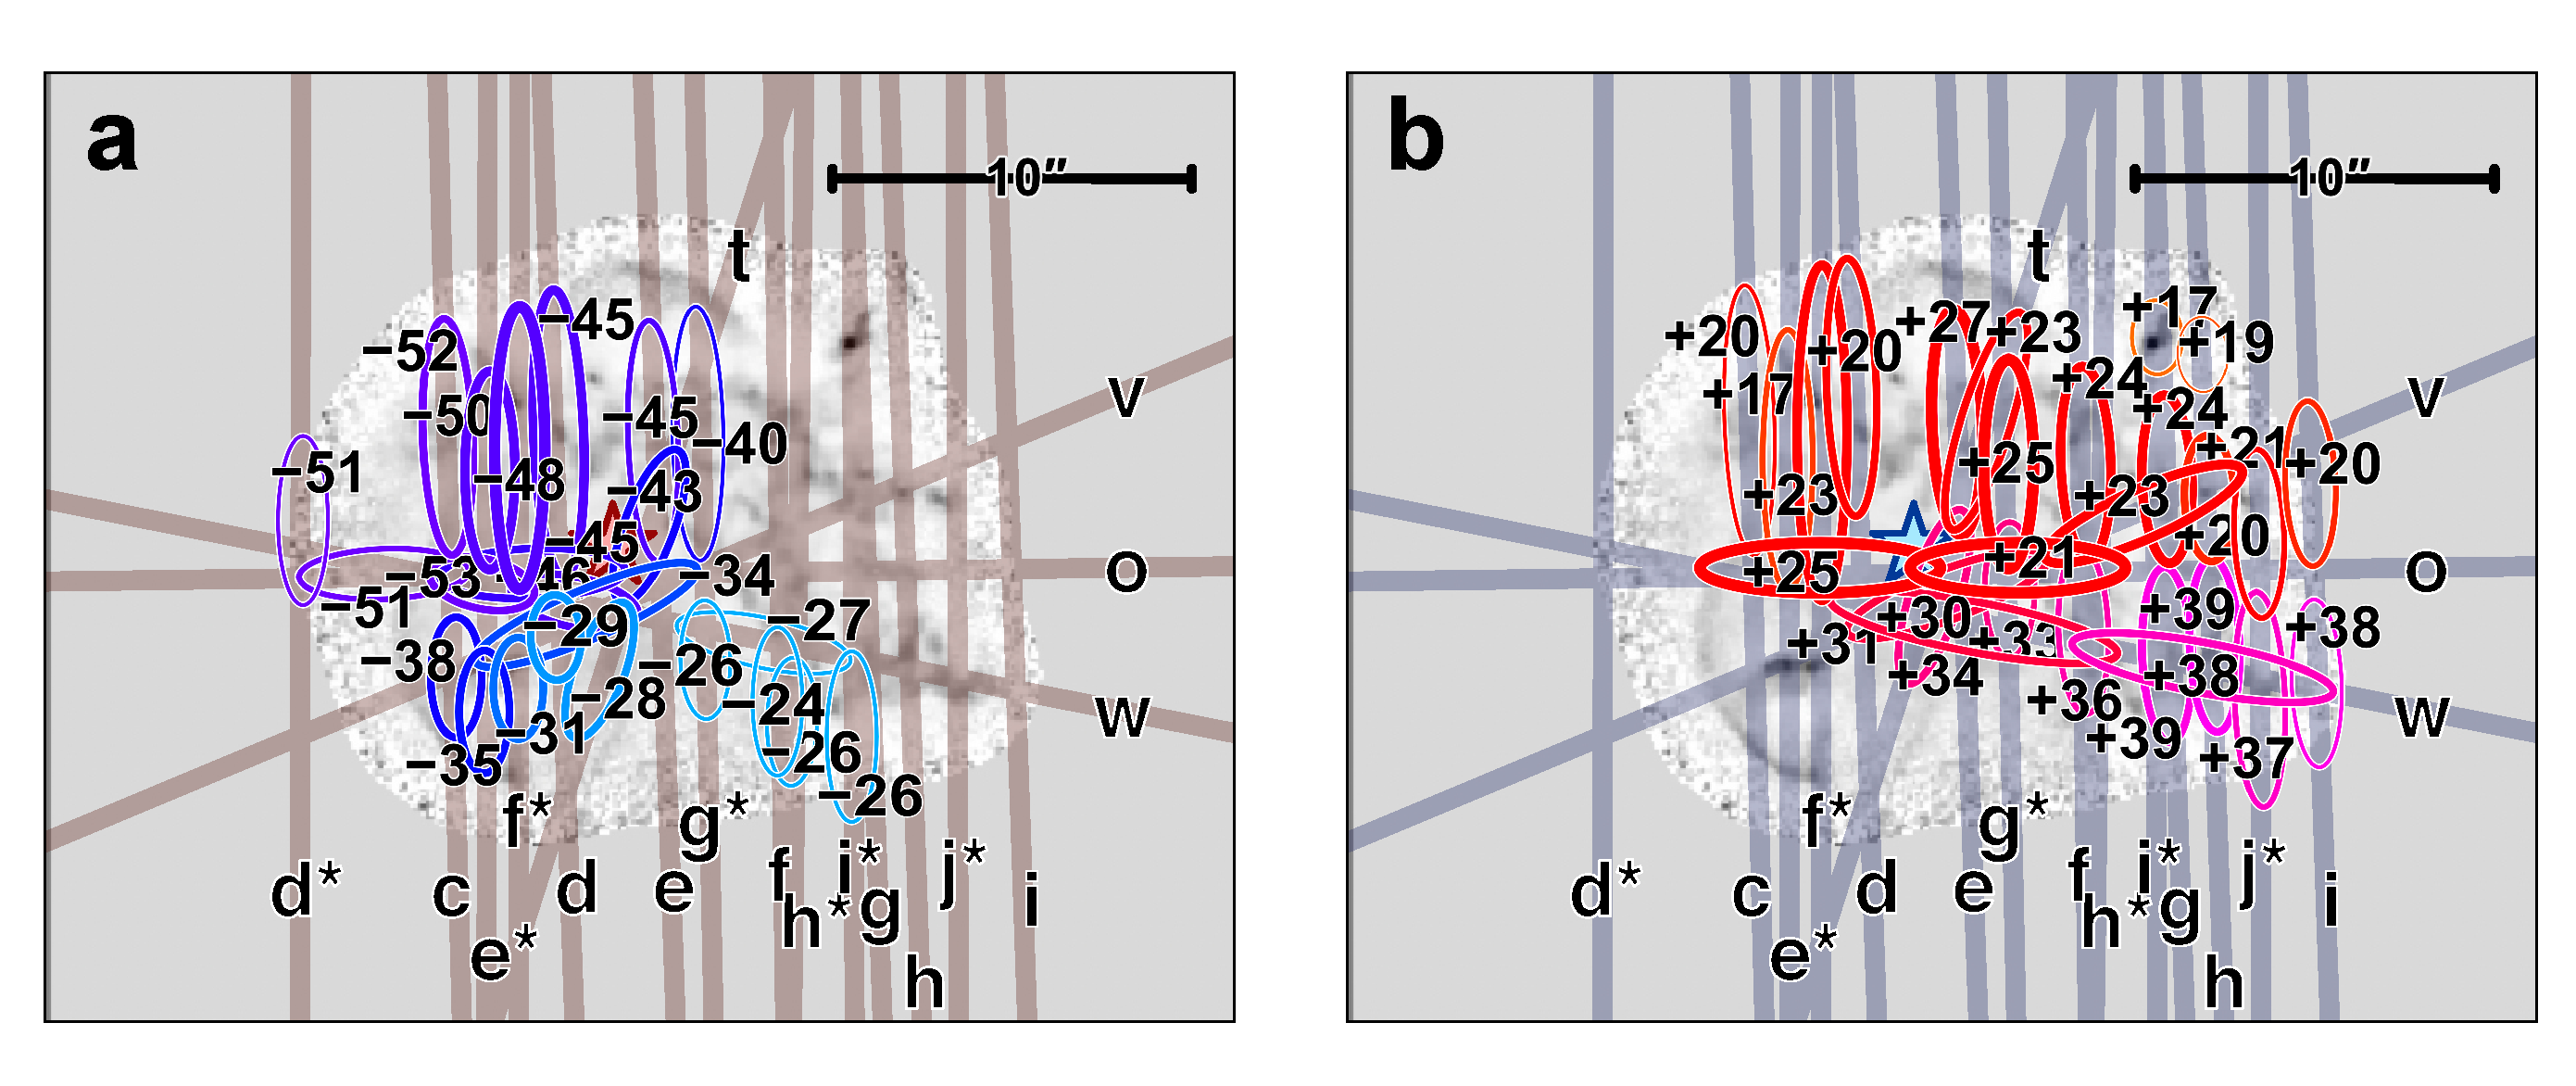
\includegraphics[width=\linewidth]{figs/turtle-knot-complex-map}
  \caption{
    Velocity features in the low-ionization knot complexes,
    which have been identified in the \nii{} slits.
    Left panel shows blue-shifted features,
    while right panel shows red-shifted features,
    each labelled with their line-of-sight velocity
    with respect to the nominal systemic velocity of \SI{40}{km.s^{-1}}.
    The line width is a qualitative indicator of the brightness of each feature.
  }
  \label{fig:knot-complex-map}
\end{figure*}

\begin{figure*}
  \centering
  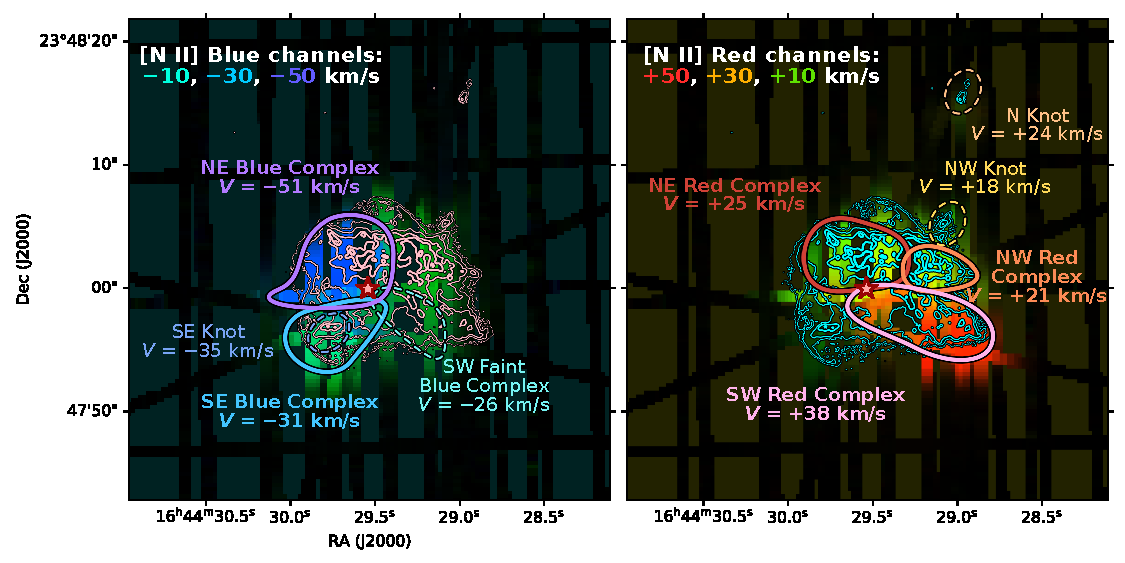
\includegraphics[width=\linewidth]{figs/turtle-nii-knot-complexes}
  \caption{
    Reconstructed velocity channel maps from the \nii{} slit spectra,
    showing the red-shifted (left panel) and blue-shifted (right panel) knot complexes.
    Note that channel maps have not been spatially interpolated,
    so that the individual slit positions can be seen.
    Each color image is constructed from 3 channels, each of width \SI{20}{km.s^{-1}},
    as indicated on the figure.
    All velocities are with respect to the nominal heliocentric systemic velocity of \SI{-40}{km.s^{-1}}.
    The low-ionization emission components from Fig.~\ref{fig:knot-complex-map}
    have been classified into 5 knot complexes,
    which are shown as colored outlines. 
  }
  \label{fig:knot-complexes}
\end{figure*}

\begin{figure}
  \centering
  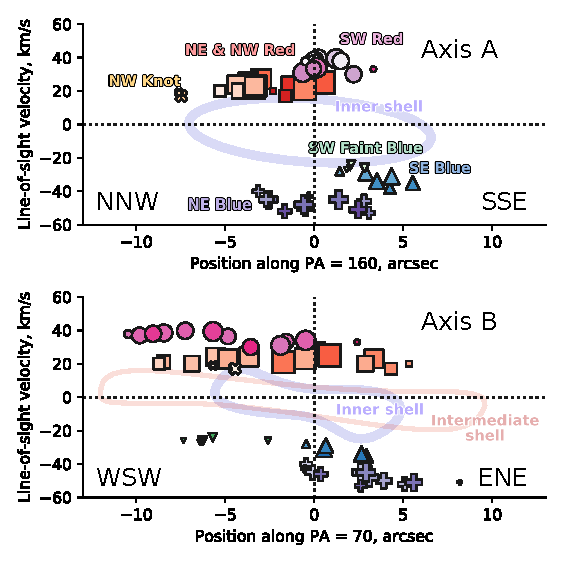
\includegraphics[width=\linewidth]{figs/turtle-knot-complexes-velocity-axes-annotated}
  \caption{
    Radial velocity versus position
    for the low-ionization features features shown in Fig.~\ref{fig:knot-complex-map}.
    Results are shown projected along along the same two axes,
    Axis~A (upper panel) and Axis~B (lower panel),
    as in Fig.~\ref{fig:shell-velocity-axes},
    but this time each feature is shown projected along both axes.
    The features are divided into different knot complexes,
    as shown in Fig.~\ref{fig:knot-complexes},
    which are indicated by symbol type and color.
    Symbol size is proportional to feature brightness (log scale)
    and symbol shade indicates position along the other axis (darker is more positive).
    Continuous lines show the same high ionization shells
    as in Fig.~\ref{fig:shell-velocity-axes}.
  }
  \label{fig:knot-complex-velocity-axes}
\end{figure}

The \nii{} emission from the nebula is dominated by small-scale knots,
as can be appreciated on the \textit{HST} images (Figure~XXX).
These knots have typical sizes \(< 1''\) and so are not spatially resolved
in our ground-based spectroscopy.
A small number of isolated knots are individually detected in our spectra,
but in general we detect only the combined emission of extended knot complexes.
Figure~\ref{fig:knot-complex-map} shows all the \nii{} emission components
identified from our spectra, but excluding those associated with the high-ionization
shells discussed above.
As previously, the components are divided into negative (left panel)
and positive (right panel) velocities.  
In Figure~\ref{fig:knot-complex-velocity-axes}
we classify the emission components into five knot complexes,
plus three individual knots, whose plane-of-sky distribution
and typical line-of-sight velocity are shown
superimposed on the \textit{HST} \nii{} image (contours)
and isovelocity channel maps reconstructed from our slit spectra (color images).

Figure~\ref{fig:knot-complexes} shows the velocity of each \nii{} component
as a function of position along the two axes that characterize the high-ionization shells:
axis~A at \(\text{PA} = \ang{160}\)
and axis~B at \(\text{PA} = \ang{70}\) (see \S~\ref{sec:high-ioniz-shells}).
The kinematics of the shells themselves are shown by faint continuous lines for comparison.
Note that the extent of the velocity axis in this figure
is twice as large as in Figure~\ref{fig:shell-velocity-axes}. 

The clearest axial alignment is seen for the SW Red complex,
which is very tightly clustered around the negative arm of axis~B.
The same is seen to a lesser extent for the NE Blue complex
around the positive arm of axis~B,
but the distribution around the axis is broader in this case.
The remaining complexes have no clear alignment with either axis,
except that the SE Blue complex is marginally more elongated
along the positive arm of axis~A.

The upper panel of Figure~\ref{fig:knot-complex-velocity-axes} indicates
that there is no clear velocity gradient along axis~A,
but the low-ionization knots have significantly faster radial velocities
than the high-ionization shells, by roughly a factor of two.
In addition, there is an asymmetry between the blue and red components:
the blue-shifted knot complexes tend to have a larger radial velocity magnitude,
but to have fainter \nii{} emission, as compared with the red-shifted knot complexes.

From the lower panel of Figure~\ref{fig:knot-complex-velocity-axes},
it is apparent that there is a significant gradient of \(\approx \SI{20}{km.s^{-1}}\)
along axis~B, which is seen in both blue-shifted and red-shifted components.
The sense of this gradient is the same as that seen in the high-ionization shells
along this axis.
It is mainly due to velocity differences
\emph{between} complexes rather than within them,
although both the SW Red and NE Blue complexes
show significant internal gradients of \(\approx \SI{10}{km.s^{-1}}\) in the same direction.

There is an approximate kinematic and spatial symmetry
between pairs of opposite knot complexes:
SW Red with NE Blue complex, and N Red with SE Blue.
It is possible that the west and east sides of the N Red complex
are actually two separate complexes,
in which case the east side would pair with the SW Faint Blue complex,
which would further reinforce this symmetry.

The knot complexes are also visible in the \oiii{} spectra,
although they are fainter than the shells in this line.
There is also a slight difference in velocity,
with \oiii{} showing expansion velocities that are \num{2} to \SI{5}{km.s^{-1}} smaller than \nii{}.
If the expansion velocities within the knot complexes are assumed to increase with radius,
then this is evidence for ionization stratification along the line of sight
with the \oiii{} emission arising slightly closer to the star than \nii{}.
This is also consistent with the HST images (e.g., Figure~\ref{fig:hst}d),
which show that the \oiii{} emission associated with the complexes is more diffuse than the compact \nii{} knots.

\subsection{Outer lobes}
\label{sec:outer-lobes}

\begin{figure*}
  \centering
  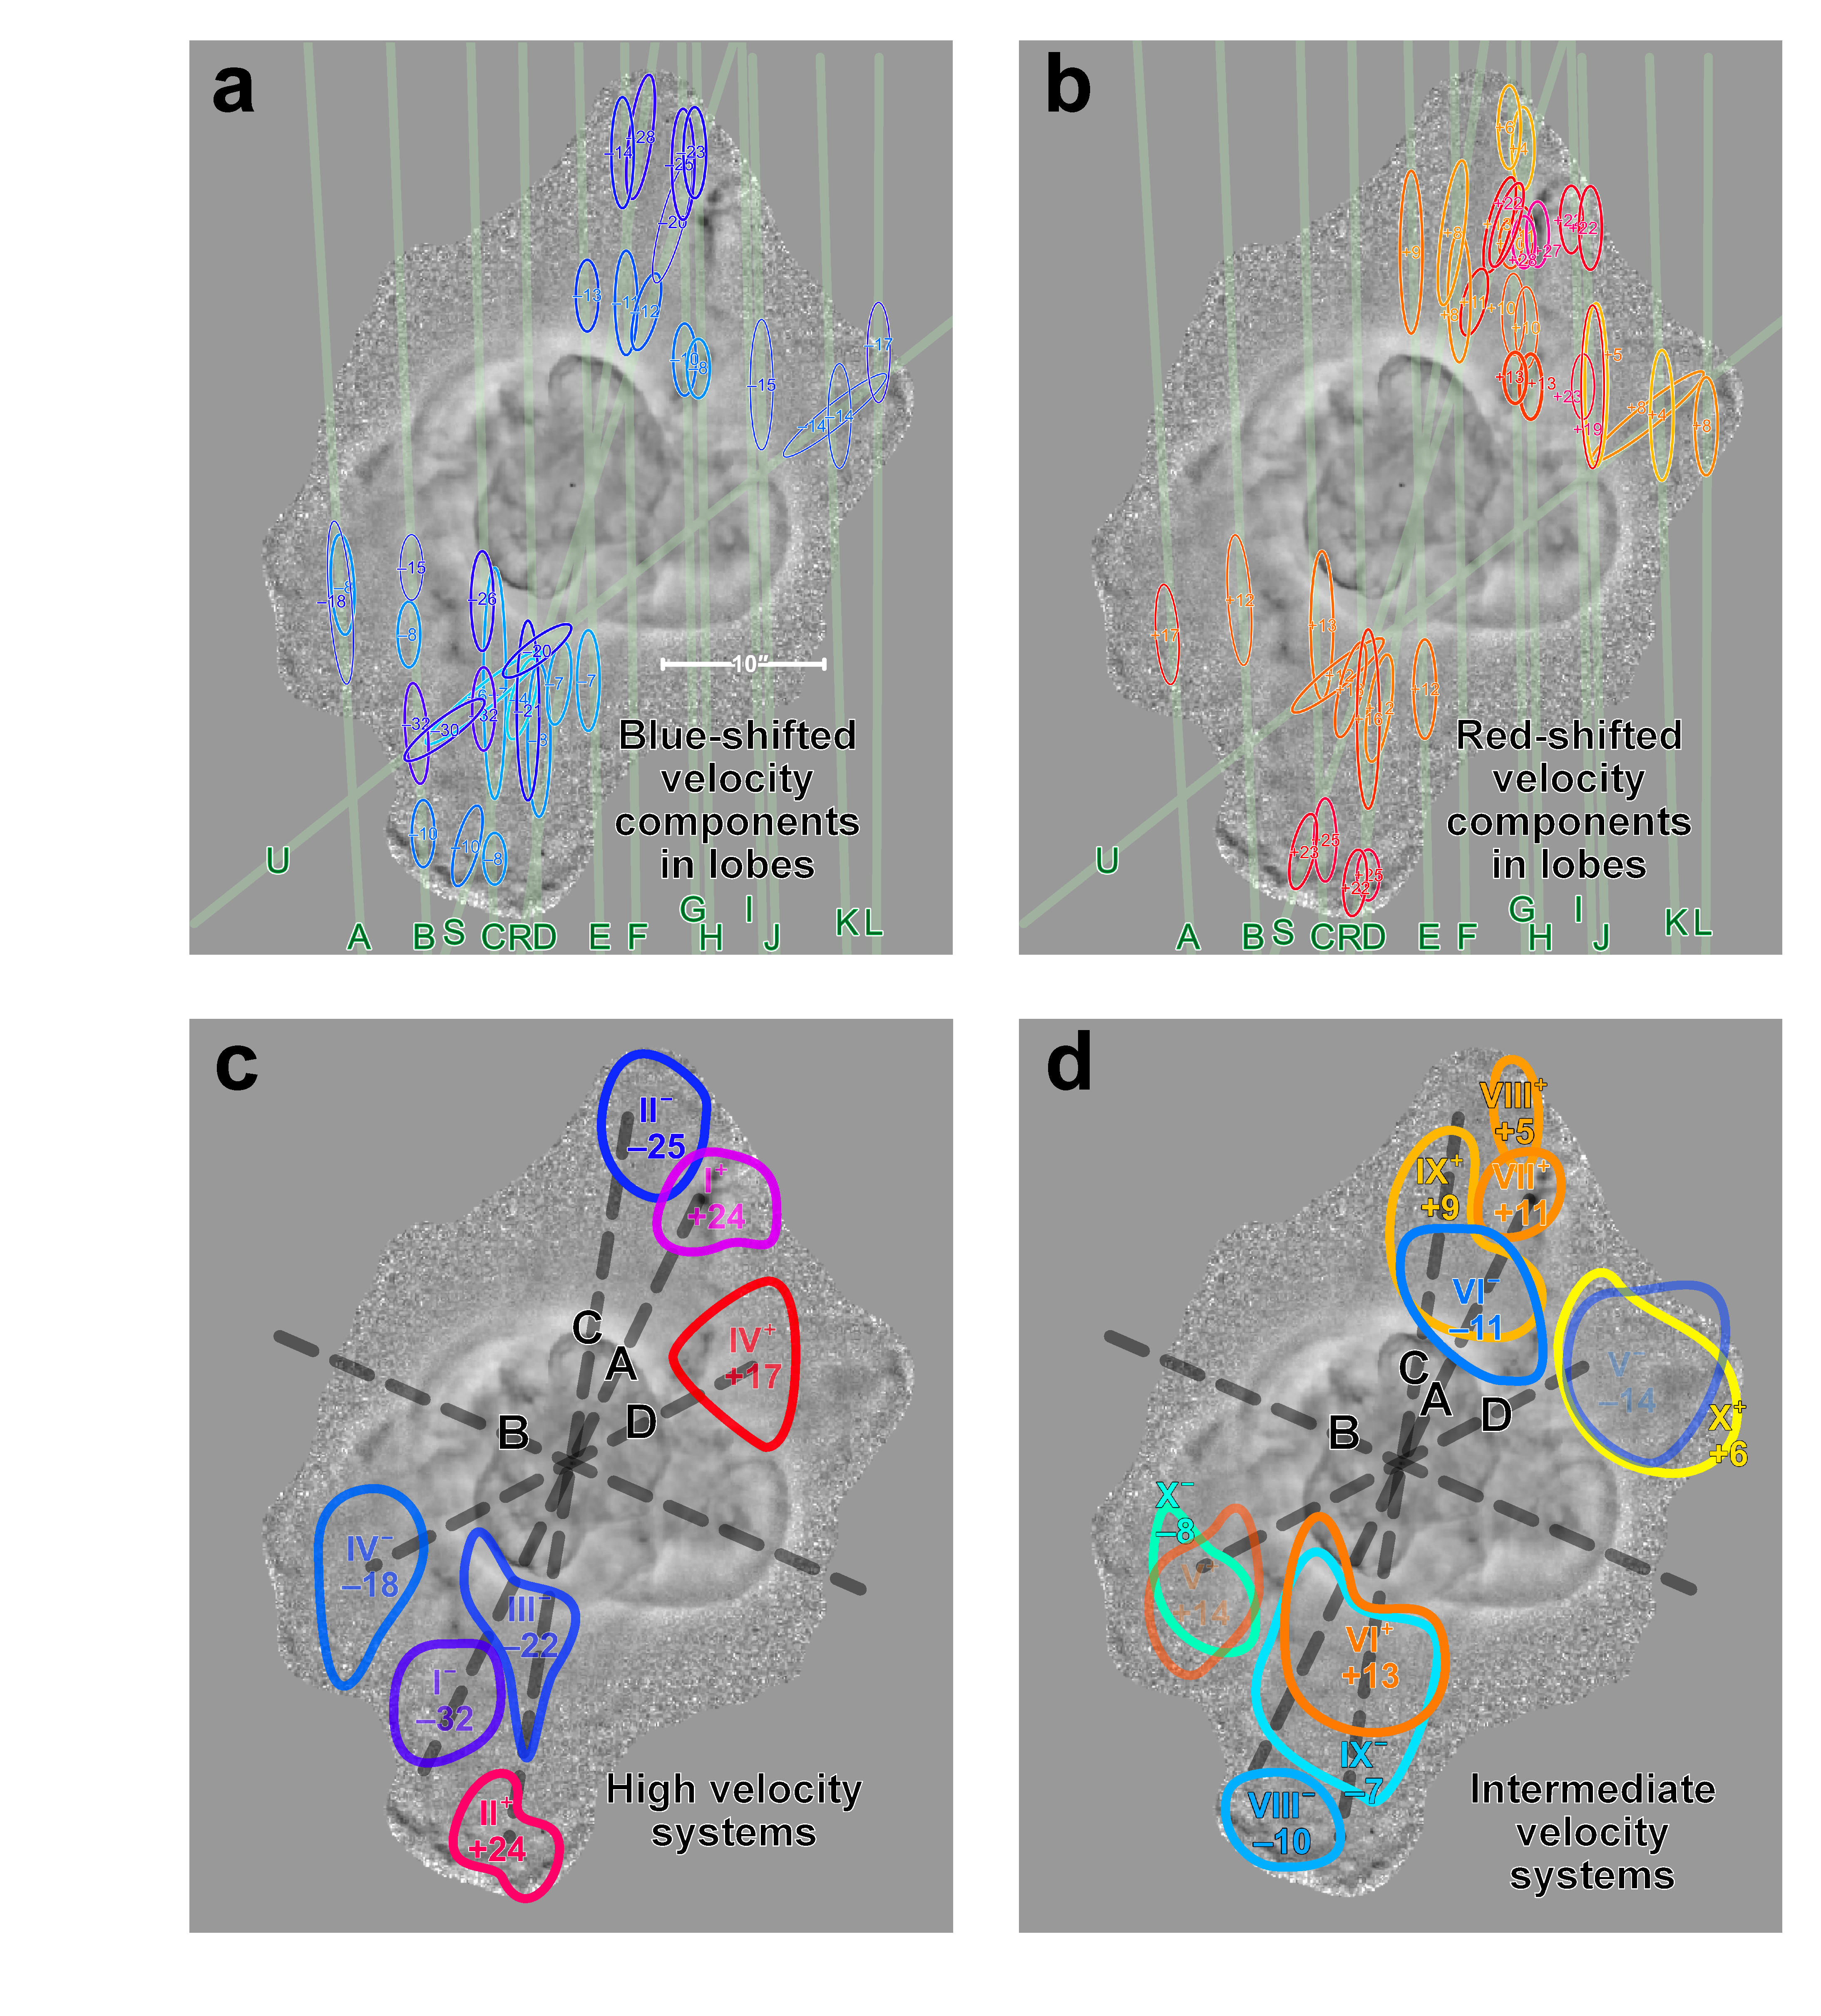
\includegraphics[width=\linewidth]{figs/turtle-lobes-simplified}
  \caption{
    Velocity components and systems in the outer lobes.
    (a)~Blue-shifted components identified in individual slits.
    (b)~Red-shifted components identified in individual slits.
    (c)~Classification of components into seven high-velocity systems (colored shapes)
    along three different axes (heavy dashed lines).
    (d)~Same but for eleven intermediate velocity systems.
  }
  \label{fig:outer-lobe-components}
\end{figure*}
\newcounter{Syscounter}
\newcommand\Sys[1]{%
  \setcounter{Syscounter}{#1}%
  \ensuremath{\mathrm{\Roman{Syscounter}}}%
}
\newcommand\SysP[1]{\ensuremath{\Sys{#1}^+}}
\newcommand\SysM[1]{\ensuremath{\Sys{#1}^-}}

The emission from the outer lobes is much fainter than the inner shells,
and is most easily detected in \oiii{}.
Figure~\ref{fig:outer-lobe-components} shows all the outer lobe velocity components
that we have been able to measure from the \oiii{} slits:
blue-shifted components in panel~a and red-shifted components in panel~b.
We have not included all of the \oiii{} components that lie outside the inner and shells, since some of these are closely associated with the low ionization knot complexes discussed above in \S~\ref{sec:knot-complexes}.
In these cases, the \oiii{} component is weaker than the corresponding \nii{} component,
slightly more spatially extended,
and with a velocity magnitude that is about \SI{5}{km.s^{-1}} smaller
(for both red and blue-shifted knots).
Such \oiii{} components are omitted from the figure 
with the exception of the N knot and the NW knot (see Fig.~\ref{fig:knot-complexes}).

As with the low-ionization knot complexes,
there are many apparent pairings between blue and red outer lobe components on opposite sides of the nebula.
This is illustrated in the lower panels of Figure~\ref{fig:outer-lobe-components},
where we classify the components into four high-velocity systems,
\Sys{1} to \Sys{4}
with \(|V| = \text{\SIrange{17}{25}{km.s^{-1}}}\) (panel~c)
and six intermediate-velocity systems,
\Sys{5} to \Sys{10}
with \(|V| = \text{\SIrange{5}{14}{km.s^{-1}}}\) (panel~d).
Nearly all of these systems have a blue and a red component
which are approximately symmetrically arranged about the central star.
For instance, the blue-shifted \SysM{2} component in the north
is paired with the red-shifted \SysP{2} component in the south.
Note, however, that \SysM{3} and \SysP{7} have no opposite counterparts.

The high-velocity systems seem to define three separate flow axes.
Most notably, system~\Sys{1}, with \(\text{PA} = \ang{155 \pm 5}\),
is closely aligned with axis~A of the high-ionization shells at \(\text{PA} \approx \ang{160}\)
(see \S~\ref{sec:high-ioniz-shells}),
and also has the same sense of inclination (receding to the north).
Although system~\Sys{2}, with  \(\text{PA} = \ang{171 \pm 5}\),
is also marginally consistent in projection with axis~A,
the sense of inclination is opposite (receding to the south),
implying that the axis is distinct,
and we name it axis~C.
System~\Sys{4}, with  \(\text{PA} = \ang{120 \pm 15}\), defines yet another axis,
which we name axis~D.
Note that none of the outer lobe components are aligned with axis~B of the high-ionization shells.

The intermediate velocity systems (Fig.~\ref{fig:outer-lobe-components}d)
are less well collimated than the high-velocity components,
but seem to be aligned with the same three axes: A, C, and D.
This is most clearly seen in the East and West Lobes,
where systems~\Sys{5} and \Sys{10} overlap the higher velocity system \Sys{4} along axis~D.
They may represent slower moving entrained material or bow shock wings from the same flow.
The same is true of the North and South Lobes,
where systems~\Sys{6}, \Sys{7}, \Sys{8}, and \Sys{9}
overlap the higher velocity systems \Sys{1} and \Sys{2}.
However, the fact that axis~A and axis~C have similar projected position angles
makes it hard to assign each intermediate velocity system to one axis or the other.


\subsection{Haloes}
\label{sec:haloes}

\begin{figure}
  \centering
  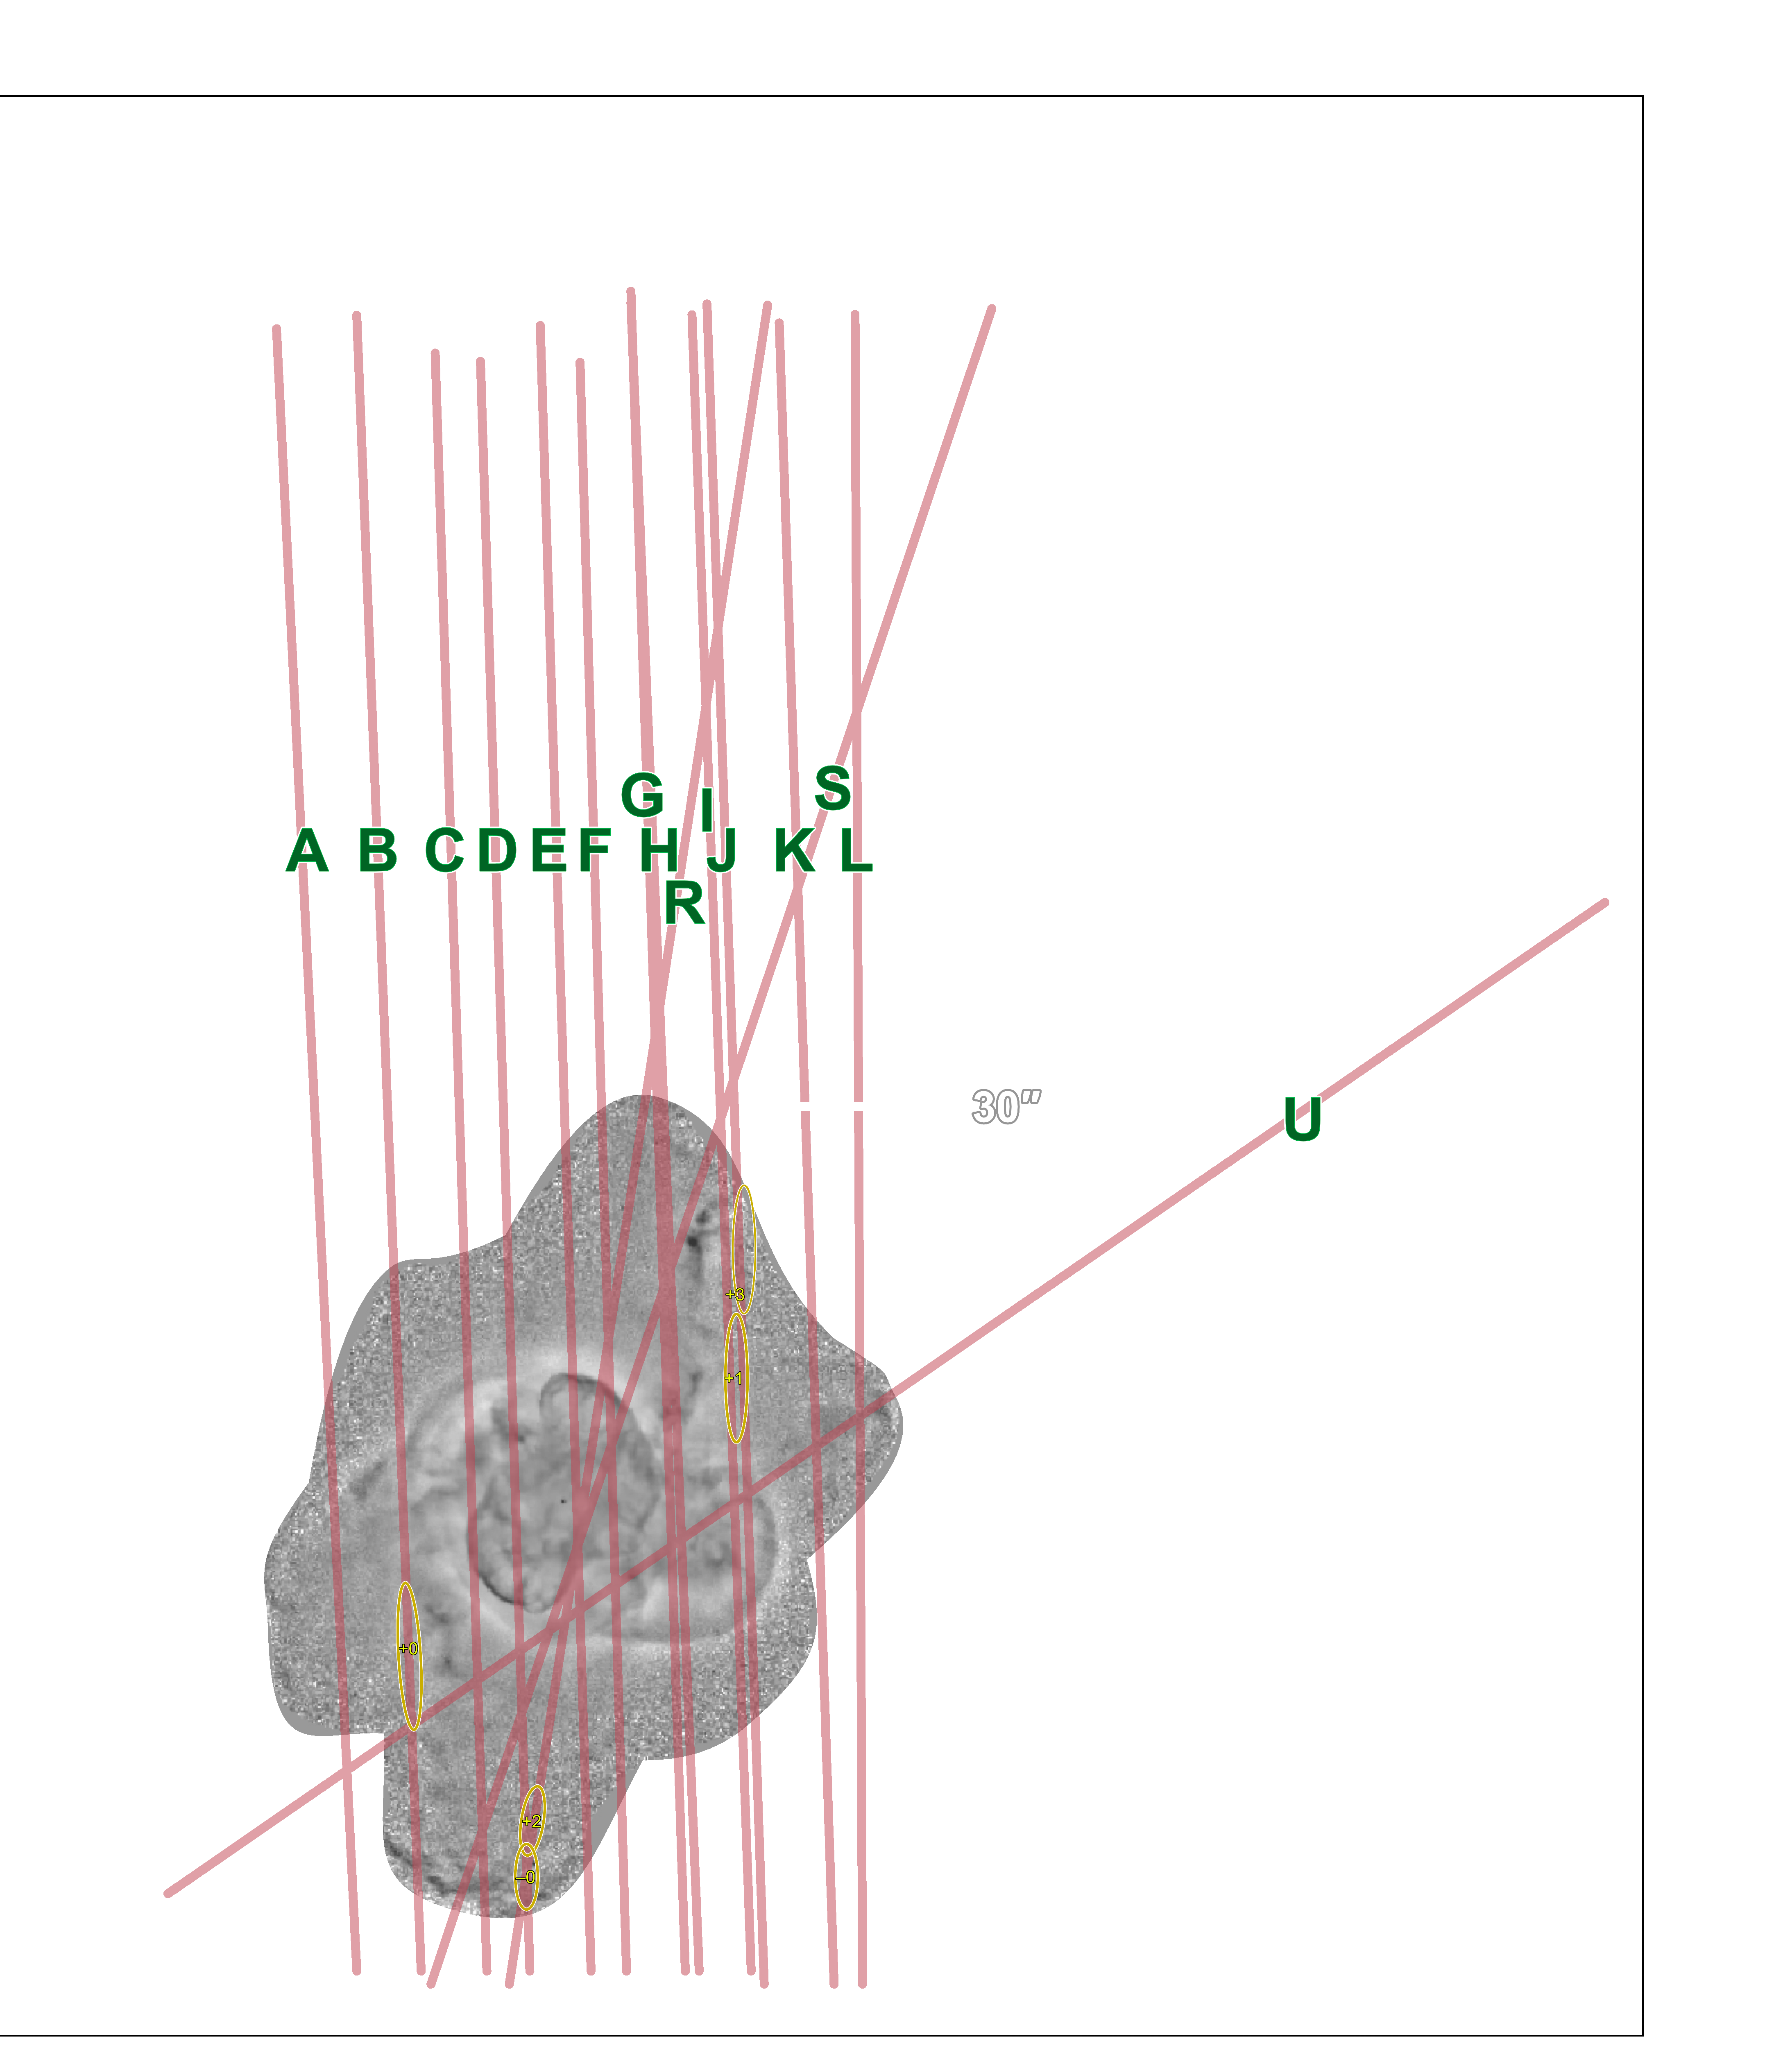
\includegraphics[width=\linewidth]{figs/turtle-halo-map}
  \caption{
    Velocity components in the halo, all measured from the \oiii{} spectra with slit positions as indicated.
    Components are divided into three classes:
    inner halo (pink ellipses), outer halo (yellow ellipses),
    and halo knots (green ellipses).
    The inner portion of the background image is
    the same high-pass-filtered \textit{HST} image
    shown in Figs.~\ref{fig:shell-velocity-components} and~\ref{fig:outer-lobe-components}.
    The outer portion of the background image is a deep \oiii{} exposure of the halo
    obtained with Mezcal in direct imaging mode (see Fig.~YYY).
  }
  \label{fig:halo-components}
\end{figure}

Figure~\ref{fig:halo-components} shows the velocity components
from the \oiii{} slits that are close to the systemic velocity,
and which are mainly associated with the nebula halo.
These components can be divided into three different types,
according to the width and location of the component.
The \textit{inner halo} (pink ellipses in the figure) is characterised by broad lines,
while the \textit{outer halo} (yellow ellipses in the figure) is characterised by narrower lines.
After correcting for instrumental broadening,
the full-width half-maximum line widths are \(W = \SI{28 \pm 2}{km.s^{-1}}\) for the inner halo,
but only \(W = \SI{14 \pm 1}{km.s^{-1}}\) for the outer halo.


The outer halo shows a smooth drop in brightness with distance
between about \(20''\) and \(30''\) from the central star,
beyond which it generally becomes undetectable in our spectra,
although it can still be seen in the very deep image shown as the background to Figure~\ref{fig:halo-components}.
Some bright emission patches are detected at larger radii
(\(40''\) to \(70''\)),
which we denote \textit{halo knots} (dark green ellipses in the figure).
These have a corrected velocity width intermediate between the inner and smooth outer halo,
\(W = \SI{19 \pm 1}{km.s^{-1}}\) but the signal-to-noise is low.

There is no clear pattern to the small velocity deviations between individual halo components,
and these are probably largely due to residual wavelength calibration uncertainties.
The mean and standard deviation for both the inner and outer halo are identical at \(V = \SI{+0.7 \pm 0.3}{km.s^{-1}}\),
which gives a more refined estimate for the heliocentric systemic velocity as
\(V_\odot = \SI{-39.3 \pm 0.3}{km.s^{-1}} \),
instead of the nominal \(\SI{-40}{km.s^{-1}}\) that we have been assuming.

Comparison of Figures~\ref{fig:outer-lobe-components} and~\ref{fig:halo-components}
shows that some inner-halo components overlap spatially with the high-velocity and intermediate-velocity systems of the outer lobes.
This is particularly true on the western side of the north and south lobes.
In these regions, there is a selection effect whereby
the halo components are more easily identifiable in regions where the outer lobe emission is weaker. 

\section{Discussion}
\label{sec:discussion}

\subsection{Velocities and positions in three dimensions}
\label{sec:veloc-posit-three}

\newcommand\AxP[1]{\ensuremath{\mathrm{#1}^+}}
\newcommand\AxM[1]{\ensuremath{\mathrm{#1}^-}}
\begin{table*}
  \caption{Positions and velocities of nebular features in three dimensions}
  \label{tab:3d}
  \centering
  %\setlength\tabcolsep{5pt}
  \sisetup{
    table-format = >2.0(1),
    table-auto-round,
  }
  \begin{tabular}{
    l % System
    S[table-format = 3.0] % PA
    r % Axis
    S % Vlos
    S % Vpos
    S % V
    S % i
    S % Rproj
    S[table-format = >1.2(2)] % R
    S[table-format = >1.1(2)] % t
    }
    \toprule
             & {PA} &        & {\(V_\text{los}\)} &  {\(V_\text{pos}\)} &  {\(V_\text{tot}\)} & {\(i\)} & {\(R_\text{proj}\)} & {\(R\)} & {\(t_\text{kin}\)}\\
    {Feature} & {\si{\degree}} & {Axis} & {\si{km.s^{-1}}}   &  {\si{km.s^{-1}}}  & {\si{km.s^{-1}}} & {\si{\degree}} & {\si{\arcsecond}} & {pc} & {\SI{1000}{yr}}\\
    \midrule
    {(1)} & {(2)} & {(3)} & {(4)} & {(5)} & {(6)} & {(7)} & {(8)} & {(9)} & {(10)} \\
    \addlinespace
    Inner shell A NNW & 340 & \AxP{A} & +8 \pm 3 & 48 \pm 7 & 49 \pm 7 & 11 \pm 4 & 7 \pm 1 & 0.07 \pm 0.01 & 1.4 \pm 0.2\\
    Outer lobe \SysP{1}/\SysP{7} & 340 & \AxP{A} & +28 \pm 2 & 82 \pm 29 & 89 \pm 27 & 22 \pm 7 & 16 \pm 1 & 0.17 \pm 0.01 & 1.9 \pm 0.7\\
    North knot & 340 & \AxP{A} & +24 \pm 1 & 60 \pm 4 & 67 \pm 4 & 26 \pm 2 & 17 \pm 1 & 0.19 \pm 0.01 & 2.7 \pm 0.2\\
    Inner shell A SSE & 160 & \AxM{A} & -17 \pm 3 & 51 \pm 7 & 55 \pm 7 & -22 \pm 4 & 7 \pm 1 & 0.08 \pm 0.01 & 1.2 \pm 0.2\\
    Outer lobe \SysM{1} & 160 & \AxM{A} & -32 \pm 1 & 71 \pm 29 & 81 \pm 26 & -28 \pm 10 & 15 \pm 2 & 0.17 \pm 0.03 & 2.0 \pm 0.8\\
    Outer lobe \SysM{8} & 160 & \AxM{A} & -10 \pm 1 & 67 \pm 9 & 68 \pm 9 & -10 \pm 2 & 23 \pm 1 & 0.23 \pm 0.01 & 3.2 \pm 0.4\\
    Outer lobe \SysP{2} & 170 & \AxP{C} & +24 \pm 2 & 58 \pm 12 & 65 \pm 11 & 26 \pm 5 & 24 \pm 1 & 0.27 \pm 0.02 & 3.9 \pm 0.9\\
    Outer lobe \SysM{2} & 355 & \AxM{C} & -25 \pm 3 &   & > 25.0 & < 0.0 & 21 \pm 3 & > 0.21 & \\
    \addlinespace
    Inner shell B ENE & 65 & \AxM{B} & -25 \pm 3 & 31 \pm 5 & 43 \pm 4 & -44 \pm 6 & 4 \pm 1 & 0.06 \pm 0.01 & 1.2 \pm 0.4\\
    NE Blue complex & 60 &  & -51 \pm 1 & 23 \pm 5 & 65 \pm 2 & -69 \pm 4 & 5 \pm 1 & 0.14 \pm 0.04 & 2.1 \pm 0.6\\
    IS ENE & 50 & \AxM{B} & -18 \pm 3 & 27 \pm 15 & 35 \pm 12 & -39 \pm 16 & 9 \pm 2 & .12 \pm 0.04 & 3.2 \pm 2.0\\
    Inner shell B WSW & 240 & \AxP{B} & +18 \pm 3 & 29 \pm 4 & 36 \pm 4 & 37 \pm 6 & 5 \pm 1 & 0.06 \pm 0.01 & 1.5 \pm 0.4\\
    IS WSW & 260 & \AxP{B} & +20 \pm 3 & 29 \pm 26 & 38 \pm 20 & 40 \pm 26 & 12 \pm 1 & 0.16 \pm 0.06 & 3.8 \pm 3.5\\
    SW Red complex & 250 &  & +38 \pm 1 & 18 \pm 3 & 49 \pm 2 & 68 \pm 3 & 7 \pm 2 & 0.19 \pm 0.06 & 3.7 \pm 1.2\\
    N(E) Red complex & 30 &  & +25 \pm 2 & 5 \pm 4 & 30 \pm 2 & 81 \pm 7 & 4 \pm 1 & 0.26 \pm 0.21 & 8.0 \pm 6.7\\
    SW Faint Blue & 225 &  & -26 \pm 1 & 26 \pm 4 & 41 \pm 3 & -50 \pm 4 & 7 \pm 1 & 0.11 \pm 0.02 & 2.6 \pm 0.5\\
    \addlinespace
    Outer lobe \SysP{10} & 285 & \AxP{D} & +6 \pm 2 & 48 \pm 43 & 49 \pm 43 & 9 \pm 8 & 19 \pm 2 & 0.19 \pm 0.02 & 3.7 \pm 3.3\\
    Outer lobe \SysP{4} & 315 & \AxP{D} & +13 \pm 1 & 33 \pm 7 & 37 \pm 6 & 25 \pm 5 & 10 \pm 1 & 0.11 \pm 0.01 & 2.9 \pm 0.6\\
    NW knot  & 310 &  & +18 \pm 1 & 11 \pm 8 & 24 \pm 4 & 63 \pm 17 & 8 \pm 1 & 0.18 \pm 0.10 & 6.7 \pm 4.5\\
    N(W) Red complex & 300 &  & +21 \pm 2 & 10 \pm 4 & 27 \pm 3 & 68 \pm 8 & 6 \pm 2 & 0.16 \pm 0.08 & 6.0 \pm 3.1\\
    Outer lobe \SysM{10} & 120 & \AxM{D} & -8 \pm 4 & 24 \pm 14 & 26 \pm 13 & -22 \pm 15 & 13 \pm 3 & 0.14 \pm 0.04 & 5.2 \pm 3.3\\
    SE Blue complex & 135 &  & -31 \pm 3 & 39 \pm 10 & 54 \pm 8 & -44 \pm 8 & 5 \pm 1 & 0.07 \pm 0.02 & 1.1 \pm 0.4\\
    SE knot & 135 &  & -35 \pm 3 & 39 \pm 10 & 57 \pm 7 & -47 \pm 8 & 8 \pm 1 & 0.09 \pm 0.02 & 1.5 \pm 0.4\\
    \bottomrule
    \multicolumn{10}{p{15cm}}{
    \textsc{Columns:}
    (1)~Name of nebular feature.
    (2)~Position angle of feature with respect to central star.
    (3)~Outflow axis that feature is best aligned with, if any.
    (4)~Line-of-sight velocity, derived from longslit spectra.
    (5)~Plane-of-sky velocity, derived from proper motions assuming \(D = \SI{2}{kpc}\).
    (6)~Total pattern velocity: \(V_{\text{tot}} = [ (1.2 V_{\text{los}})^2 + V_{\text{pos}}^2 ]^{1/2}\) (see text for explanation of the factor 1.2).
    (7)~Inclination of velocity vector to line of sight: \(\tan i = 1.2 V_{\text{los}} / V_{\text{pos}}\).
    (8)~Projected radius of feature from central star.
    (9)~True radius, assuming that velocity vector is strictly radial: \(R = R_{\text{pos}} / \cos i\).
    (10)~Kinematic timescale: \(t_{\text{kin}} = R_{\text{pos}} / V_{\text{pos}}\).
    }
  \end{tabular}
\end{table*}

For those nebular features where both proper motion and radial velocity measurements exist,
it is possible to estimate the full three-dimensional velocity vector.
Under the assumption that all motions are strictly radial,
one can also find the three-dimensional position.
These are given in Table~\ref{tab:3d} for a wide variety of nebular features
in the inner shells, intermediate shell, low-ionization knots, and outer lobes.\footnote{
  Note that the uncertainties given in the table are derived from observational errors only,
  and they do not include the systematic uncertainty in the distance.
}

When combining radial velocities and proper motion measurements,
it is necessary to account for the fact that radial velocities measure the material speed,
whereas proper motions measure pattern speeds of shocks or ionization fronts \citep{Mellema:2004a}. 
The exact correction factor (material speed divided by pattern speed)
is model-dependent (e.g., Appendix~A of \citealp{ODell:2009c}),
but is predicted to be generally larger than unity
\citetext{see Fig.~8 of \citealp{Jacob:2013a}}
unless the nebula is in the recombination phase.
For simplicity, we adopt a constant correction factor of 1.2 for all entries in Table~\ref{tab:3d},
which is consistent with the predicted value for expansion velocities greater than \SI{30}{km.s^{-1}}
\citetext{see Fig.~3 of \citealp{Schonberner:2019a}}.

\begin{figure*}
  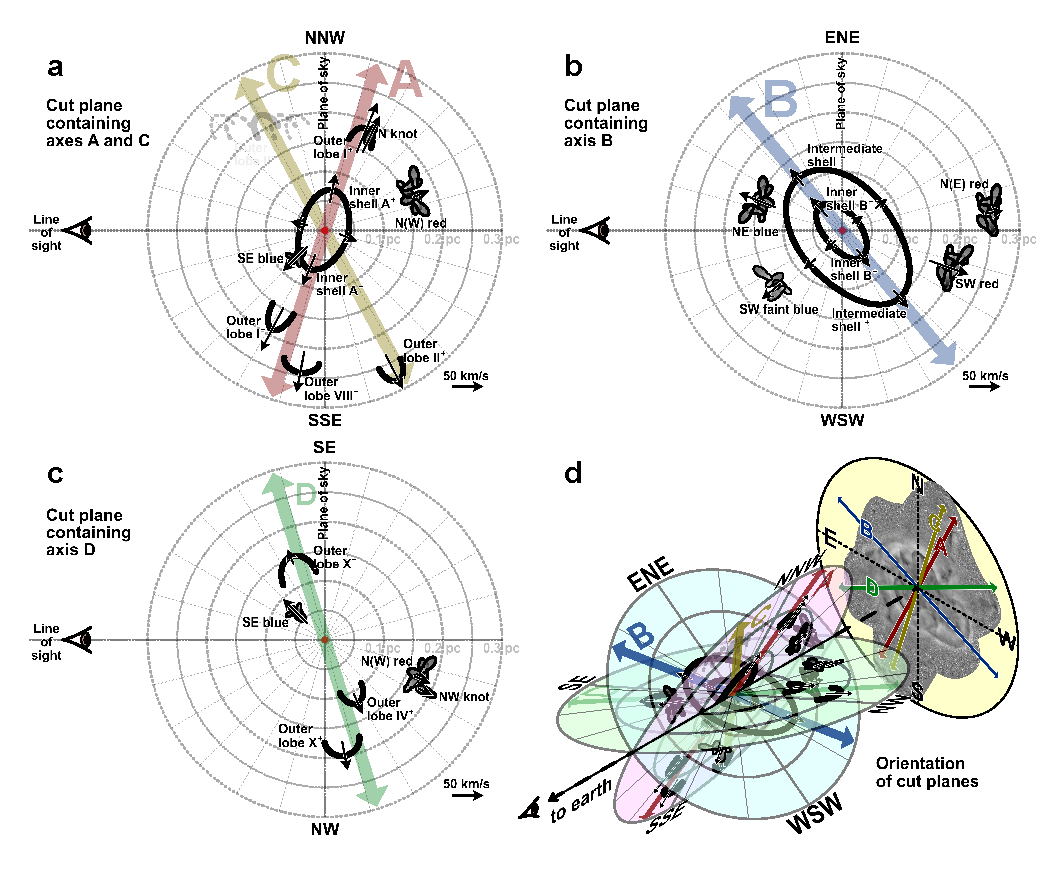
\includegraphics[width=\linewidth]
  {figs/cut-axis-4panel}
  \caption{Three dimensional reconstruction of the nebular structure and kinematics. }
  \label{fig:cut-axis-3d}
\end{figure*}

An approximate three-dimensional visualization of the nebular structure is given in Figure~\ref{fig:cut-axis-3d}.
The three axes, A, C, and D, that define the outer lobes all have small inclinations,
\(|i| < \ang{30}\) to the plane of the sky,
while the knot complexes all have higher inclinations,
\(|i| > \ang{45}\).

It is apparent from this figure that the three axes that define the outer lobes,
A, B, and D,
can be grouped into a loose conical structure with a half-opening angle of 
\begin{figure}
  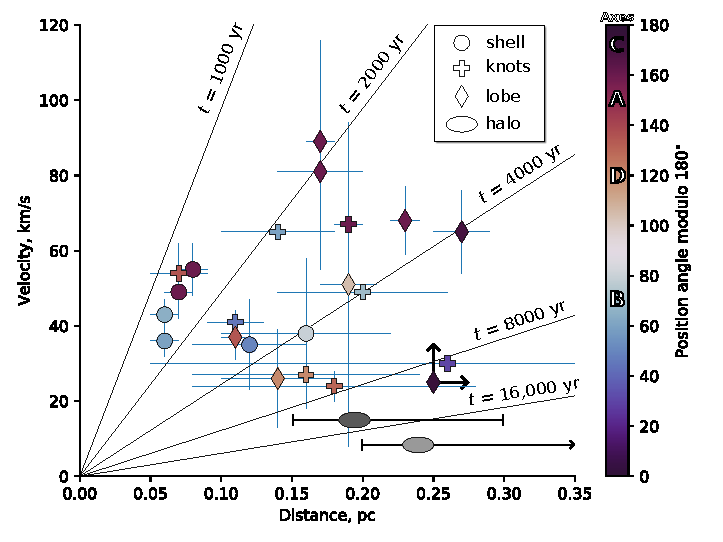
\includegraphics[width=\linewidth]
  {figs/vel-radius-systems-annotated.pdf}
  \caption{
    True velocity, \(V_{\text{tot}}\), versus true radius, \(R\), for all the features listed in Table~\ref{tab:3d}.
    Diagonal lines show dynamical times between \num{1000} and \SI{16000}{years}, as marked.
    Symbol shape indicates the type of feature:
    circle symbols are high-ionization shells (\S~\ref{sec:high-ioniz-shells}),
    cross symbols are low-ionization knots or knot complexes (\S~\ref{sec:knot-complexes}),
    diamond symbols are high-velocity and intermediate-velocity systems in the outer lobes (\S~\ref{sec:outer-lobes}).
    Error bars show the observational uncertainties given in the table,
    except for outer lobe system \SysM{2}, where the lack of proper motion measurements mean that only lower limits for \(V_{\text{tot}}\) and \(R\) are available, indicated by arrows.
    The color of each symbol corresponds the position angle of the feature, as shown by the key at right,
    which also indicates the values for each of the four axes: A, B, C, and D.
    The position angle is calculated modulo \ang{180} so that the positive and negative arm of each axis have the same color.
    Also shown (gray ellipses) are the expansion velocity and range of radii of the inner and outer halo features (\S~\ref{sec:haloes}).
      }
  \label{fig:ages}
\end{figure}



\subsection{Density structure of the nebula}
\label{sec:density-structure}

\begin{table*}
  \caption{Physical parameters of nebular components}
  \label{tab:summary}
  \begin{tabular}{
    l % Component
    r % Ha flux
    r % Density
    S % Mass
    r % ioniz param
    S % tstart
    S % tstop
    S % Mdot
    r % Vel
    }
    \toprule
    {}          & {\Ha{} flux} & {Ionized Density} & {Ionized Mass}    & {Ionization Parameter} & {\(t_{\text{start}}\)} & {\(t_{\text{end}}\)} & {\(\dot{M}\)} & {\(V\)}\\
    {Component} & {\% of total}& {\si{H.cm^{-3}}} & {\(M_\odot\)} &          & {\SI{1000}{yr}}      & {\SI{1000}{yr}}    & {\si{\msun.yr^{-1}}} & {\si{km.s^{-1}}}\\
    \midrule
    {(1)} & {(2)} & {(3)} & {(4)} & {(5)} & {(6)} & {(7)} & {(8)} & {(9)}\\
    \addlinespace
    Inner shells & 44\% & 4000--5000 & 0.078 & 0.0036--0.0070 & -4 & -1.5 & 3.1e-5 & 40--55\\
    Intermediate shell & 13\% & 700--1000 & 0.135 & 0.0080--0.0140 & -10 & -4 & 2.3e-5& 35--38\\
    Knot complexes & 42\% & 2000--5000 & 0.063 & 0.0004--0.0050 & -8 & -1.5 & 9.7e-6& 24--67\\
    Outer Lobes & 1\% & 160--320 & 0.024 & 0.0086--0.0224 & -5 & -2 & 8e-6 & 40--90\\
    Inner Halo & 0.5\% & 80--160 & 0.030 & 0.0200--0.0340 & -20 & -10 & 3e-6 & 15: \\
    Outer Halo & 0.2\% & 15--40 & 0.042 & 0.0540--0.0760 & -40 & -20 & 2.1e-6 & 7: \\
    \addlinespace
    NW knot & 0.01\% & 6700 & 1e-5 & 0.0006 & -7.1 & -6.7 & 2.5e-8 & 24\\
    SE knot & 0.08\% & 8200 & 6e-5 & 0.0034 & -1.25 & -0.95 & 2e-7 & 54\\
    N knot &  0.02\% & 3000 & 3e-5 & 0.0012 & -3.0 & -2.7 & 1e-7 & 67\\
    \bottomrule
  \end{tabular}
\end{table*}

To further investigate the structure of NGC~6210,
we have used HST WFPC2 narrow-band images to derive the surface brightness in the lines \Ha{} \Wav{6563}, \Hb{} \Wav{4861}, \nii{} \Wav{6583}, and \oiii{} \Wav{5007}.
Flux calibration is carried out following the procedure outlined in \citet{Rubin:2002a}, which accounts for contamination of each emission line filter by non-target lines and atomic continuum emission \citetext{see also \citealp{Ueta:2019a}}.
Foreground dust extinction is corrected for using the observed Balmer decrement, \(\Ha/\Hb\),
assuming an intrinsic value of 2.85 and the reddening law of \citet{Cardelli:1989a},
yielding an average extinction of \(C(\Hb) = 0.13\) for the nebula.
The total intrinsic \Ha{} flux for the nebula is then found by summing over the entire HST image,
yielding \(F(\Ha) = \SI{3.176e-10}{erg.s^{-1}.cm^{-2}}\),
which is almost identical to that found by previous studies \citep{Liu:2004a}.

For each of the nebular features listed in Table~\ref{tab:3d},
we have measured the \Ha{} surface brightness \(S(\Ha)\) and flux \(F(\Ha) = S(\Ha)\,d\Omega\),
where \(d\Omega\) is the solid angle of each feature.
Results aggregated by type of feature are presented in the upper section Table~\ref{tab:summary}.
Column~2 gives the fraction of the total \Ha{} flux due to each component,
which is dominated by roughly equal contributions from the high-ionization inner shells and the low-ionization knot complexes, summing to over 85\% of the total.

\begin{figure}
  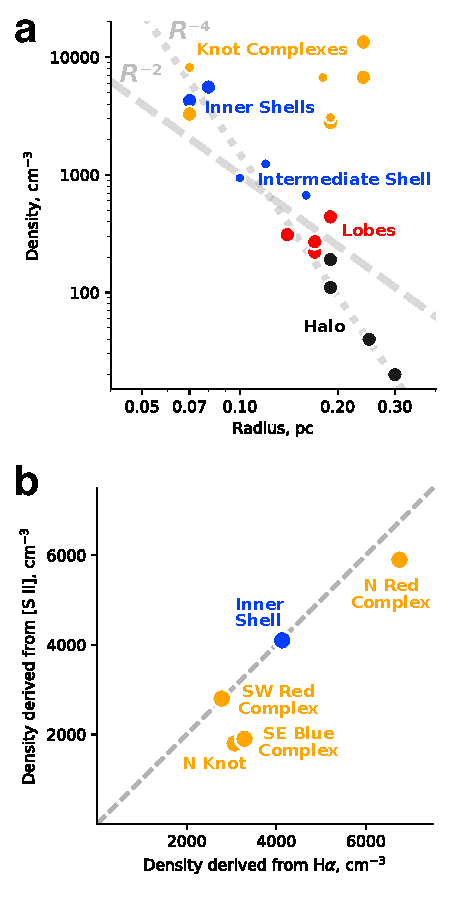
\includegraphics[width=0.8\linewidth]
  {figs/turtle-density-combined}
  \caption{
    (a)~Ionized density of different nebular features as a function of true distance from the central star.
    Densities are derived from the \Ha{} surface brightness, as explained in the text,
    and distances are deprojected using the kinematic information of Table~\ref{tab:3d}.
    Gray lines show power-law density distributions of \(n \propto R^{-2}\) (dashed)
    and \(n \propto R^{-4}\) (dotted).
    (b)~Comparison between densities derived from \Ha{} surface brightness and densities derived from the \sii{} 6716/6731 line ratio for the small number of features that are detected in our single Mezcal \sii{} slit spectrum. 
      }
  \label{fig:density-plots}
\end{figure}

Assuming a homogeneous fully-ionized emission region of hydrogen density \(n\) and line-of-sight depth \(dz\), the \Ha{} surface brightness due to recombinations is predicted to be 
\begin{equation}
  \label{eq:sha-density}
  S(\Ha) = \frac{1.0932\, \alpha_{\text{eff}}\, E(\Ha) \, n^2 \, dz} {4\pi}
  % n = \left( \frac{4\pi\, S(\Ha)}{\alpha_{\text{eff}}\, E(\Ha)\,dz } \right)^{1/2}
\end{equation}
where \(\alpha_{\text{eff}} = \SI{8.6e-14}{cm^{3}.s^{-1}}\) is an effective recombination coefficient \citep{Osterbrock:2006a}%
\footnote{We assume \(T = \SI{9500}{K}\) and that the Lyman lines are optically thick, while the Lyman continuum is optically thin, as appropriate for a matter-bounded nebula.}
and \(E(\Ha) = h c / \lambda = \SI{3.027e-12}{erg}\).
The factor \num{1.0932} accounts for the free electron contribution from Helium, assumed to be singly ionized.
Therefore, if \(dz\) can be determined for each feature, then the ionized density follows as \(n \propto [S(\Ha) / dz]^{1/2}\).
We estimate \(dz\) differently for knot-like and shell-like features.
For the first, we take \(dz = (dr\, ds)^{1/2}\), where \(dr\) is the projected width of the knot in the radial direction and \(ds\) is the width in the transverse direction.
For the second we take the maximum chord length of the shell, calculated as \(dz = 2 [R_c^2 - (R_c - dr)^2]^{1/2}\), where \(R_c\) is the shell radius of curvature and \(dr\) is the shell thickness
(limiting cases are \(dz \approx 2 R_c\) for thick shells and \(dz \approx 2 (2 R_c\, dr)^{1/2}\) for thin shells).

Resultant densities are shown in column~3 of Table~\ref{tab:summary} and are plotted against true (deprojected) radius in Figure~\ref{fig:density-plots}a.
It can be seen that a very wide range of densities is present in the nebula, from \(\approx \SI{4000}{cm^{-3}}\) in the inner shells and knot complexes down to \(\approx \SI{30}{cm^{-3}}\) in the outer halo.
For most components, there is a consistent steep decline of density with radius,
which is well approximated by \(n \propto R^{-4}\) (gray dotted line in the figure).
The exception to this rule is the outlying low-ionization knots,
located at about \SI{0.2}{pc} from the star, which have a density 20--50 times higher than the other components at a comparable radius.

As a check on our \Ha{}-derived densities, we also calculate densities from Mezcal observations of the red \sii{} doublet for a single slit position (Slit~S of Fig.~2).
This passes through five distinct spatio-kinematic features in the inner nebula,
allowing us to measure the line ratio \(I(6716)/I(6731)\) for each
(unfortunately, \sii{} emission from the outer lobes and halo is undetectably weak).
Because the relative spectrograph efficiency between the doublet wavelengths is not well-determined,
we have calibrated the line ratios by forcing the average value over the entire slit to be \(I(6716)/I(6731) = 0.60\), in agreement with the spectrophotometry of \citet{Liu:2004a}.
Results are shown in Figure~\ref{fig:density-plots}b,
calculated with PyNeb \citep{Luridiana:2015a} using atomic data from \citet{Podobedova:2009a} and \citet{Tayal:2010a}.
It can be seen that there is a reasonable agreement between the two density diagnostics,
which justifies our decision not to use any filling factor correction in equation~\eqref{eq:sha-density}.
The need for a filling factor is obviated by carefully calculating the line-of-sight depth of each emission component separately.


\subsection{Reconstructed mass-loss history}
\label{sec:reconstr-mass-loss}

Once the density is known, then the column density of ionized hydrogen follows as proportional to \(S(\Ha)/n\) and 
the ionized mass of each component can be calculated as
\begin{equation}
  \label{eq:mass}
  M = \frac{4\pi D^2\, \bar{m}\, F(\Ha) }{\alpha_{\text{eff}}\, E(\Ha)\, n} \ , 
\end{equation}
where \(D\) is the distance from Earth (assumed \SI{2}{kpc}) and \(\bar{m} \approx \SI{2.17e-24}{g}\) is the mean mass per hydrogen nucleon.
The total ionized mass of the nebula is found to be \SI{0.372}{\msun} and results for individual components are shown in column~4 of Table~\ref{tab:summary}.
It is interesting to note that the high-density components (inner shell plus knot complexes)
only represent about one-third of the total ionized mass,
despite dominating the emission line flux.
The intermediate shell is the most massive single component (\SI{0.135}{\msun}),
also roughly one-third of the total,
with the remaining third corresponding to the outer lobes and halos.

\begin{figure}
  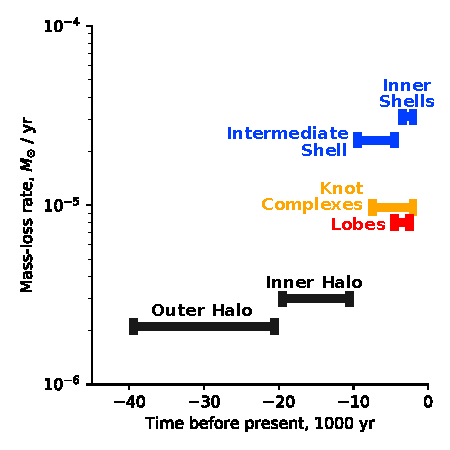
\includegraphics[width=\linewidth]
  {figs/mass-loss-history-annotated}
  \caption{
    Reconstruction of the mass-loss history of NGC~6210.
    Horizontal bars show the time period and mass-loss rate that led to the formation of each nebular component, as labeled.
    Only the average mass-loss rate is shown,
    although for the cases of the knot complexes and lobes the ejection was highly intermittent and non-isotropic during the indicated period.
    The red vertical line shows the end of the period of high mass-loss.
    Since then, the mass loss rate has declined to a much lower value. 
      }
  \label{fig:mass-loss-history}
\end{figure}


The masses can be combined with the kinematic ages (column~10 of Table~\ref{tab:3d}) to estimate the mass loss history of the nebula.
This is given in columns~6 to~8 of Table~\ref{tab:summary} and illustrated in Figure~\ref{fig:mass-loss-history}.
For the start and end times of each component, we take the full range of kinematic times of discrete features in the case of the lobes and knot complexes.
In the case of shells, the start time is taken as the kinematic age of material just outside the shell (for instance, the innermost halo material in the case of the intermediate shell).
In all cases, it is implicitly assumed that no significant acceleration or deceleration has taken place,
which may not be accurate, especially for the inner shells that have been shocked due to the action of the fast wind.
In general, the mass loss is seen to increase monotonically over the last \SI{40000}{yr} from about \SI{2e-6}{\msun.yr^{-1}} to about \SI{3e-5}{\msun.yr^{-1}} in the last few thousand years.
Note that the values shown in Figure~\ref{fig:mass-loss-history} are average values over the respective periods,
so the sudden jump that is apparent \SI{10,000}{yr} ago may have been a more gradual transition.
Also, this method can only estimate mass loss before \SI{1500}{yr} ago, which is the kinematic timescale of the inner shells.
Since that time, the mass-loss rate is expected to have declined significantly
due to the central star transitioning to higher effective temperature and smaller radius,
eventually reaching the present-day value of \(\dot{M} = \SI{9.12e-9}{M_\odot.yr^{-1}}\) at a wind velocity of \(V = \SI{2150}{km.s^{-1}}\) \citep{Herald:2011a}.
This is indicated on the figure by the gray downward pointing arrow.


\subsection{Ionization structure of the nebula}
\label{sec:ioniz-struct-nebula}

\begin{figure}
  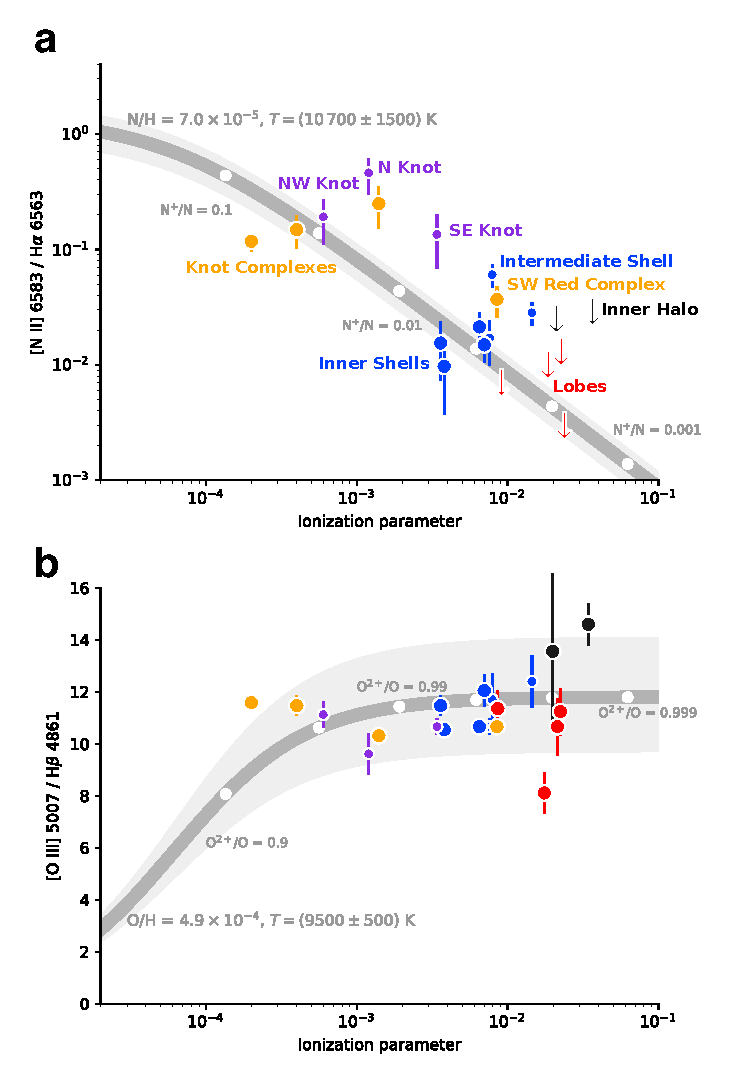
\includegraphics[width=\linewidth]
  {figs/line-ratios-vs-ion-parameter}
  \caption{
    Diagnostic line ratios plotted against ionization parameter for different nebular features:
    (a)~\nii/\Ha, (b)~\oiii/\Hb.
    Large yellow symbols show knot complexes and small yellow symbols show individual knots, as labeled.
    Large blue symbols show the inner peanut shells, and small blue symbols show the intermediate shell.
    Red symbols show the outer lobes and black symbols show the halo.
    Since the \nii{} line is not detected from the lobes and halo,
    only upper limits are available for these components in panel~a.
    The ionization parameter is calculated from the \Ha{} surface brightness and the three-dimensional reconstruction, as explained in the text.
    The thick gray line in each panel shows a toy model of fixed elemental abundance and temperature as labeled,
    with varying ion fraction as determined by optically thin photoionization equilibrium as a function of ionization parameter.  
      }
  \label{fig:line-ratios}
\end{figure}

There is a marked difference in appearance of the nebula between
high-ionization lines such as \oiii{} (Fig.~\ref{fig:proper-motions-oiii})
and low-ionization lines such as \sii{}, \oii{} and \nii{} (Fig.~\ref{fig:proper-motions-nii}),
implying that there are strong variations in the degree of ionization.
The appearance in \Ha{} is broadly similar to \oiii{},
which suggests that the doubly ionized ions, such as \chem{O^{2+}} and \chem{N^{2+}},
are the dominant stages,
whereas the singly ionized ions, such as \chem{O^{+}} and \chem{N^{+}},
have low abundance in most of the nebula.
This in turn implies that the nebula must be optically thin in the \chem{H^0} and \chem{He^0} ionizing continua,
which is also consistent with the fact that the \nii{} emission is \emph{not} concentrated in an outer ring,
as would be expected for an optically thick nebula
\citetext{for example, the Ring Nebula, \citealp{ODell:2013b}}.

\newcommand\Fion{\ensuremath{F_{\text{ion}}}}
\newcommand\ionpar{\ensuremath{U_{\text{ion}}}}
In an optically thin nebula, the flux of ionizing photons at each point is \(\Fion = Q / 4\pi R^{2}\),
where \(Q\) is the ionizing photon luminosity.
The local ionization parameter is defined as \(\ionpar = \Fion / n c\), where \(c\) is the speed of light. 
We have calculated \(\ionpar\) for each of the features listed in Table~\ref{tab:3d}
and list in column~5 of Table~\ref{tab:summary} the range of values found for each component.
In this calculation, we use the density of each feature as calculated from the \Ha{} surface brightness (\S~\ref{sec:density-structure})
and assume \(Q = \SI{4.9e47}{s^{-1}}\), which we derive from the CSPN stellar atmosphere models of \citet{Krticka:2020a} using the stellar parameters of \citet{Herald:2011a}.
In Figure~\ref{fig:line-ratios} we plot the line ratios \nii{} \Wav{6583}/\Ha{} and \oiii{} \Wav{5007}/\Hb{} against the ionization parameter for each feature.
The \nii{} and \oiii{} surface brightness were determined from HST images, as outlined in \S~\ref{sec:density-structure}.

It is apparent from the table and figure that there is a wide range of ionization parameters in the nebula.
The steep decline in density with radius (faster than \(R^{-2}\)) means that the ionization parameter tends to increase with radius, although the lowest values are associated with the knot complexes, owing to their relatively high densities as compared with other features at similar radii.
Figure~\ref{fig:line-ratios} shows that the \nii/\Ha{} ratio varies by two orders of magnitude and is clearly anti-correlated with \ionpar.
The \oiii/\Hb{} ratio, on the other hand, shows no correlation with \ionpar{} and indeed varies little within the nebula.
This is what is expected in an optically thin nebula, where the doubly ionized metals predominate.

As an example, gray solid lines in Figure~\ref{fig:line-ratios} show a toy photoionization model,
in which we assume
\(
\chem{O^{2+}} / \chem{O^+} = \chem{N^{2+}} / \chem{N^+} = A \, \ionpar ,
\)
where \(A \approx \num{1.6e4}\) is a dimensionless constant,
whose value we fix by requiring the model to approximately fit the \(\nii/\Ha\) observations.\footnote{
  Setting the \chem{N} and \chem{O} ion fractions to be equal in this equation is tantamount to assuming an \chem{N^+/O^+} ionization correction factor (ICF) of unity \citep{Kingsburgh:1994a}.
  Fits to a large suite of photoionization models
  \citetext{equations~[14--16] of \citealp{Delgado-Inglada:2014b}}
  imply \(\chem{ICF(N^+/O^+)} = 1.4 \pm 1.0\) for the nebular parameters of NGC~6210,
  whereas spectrophotometry of the whole nebula \citep[Table~7]{Pottasch:2009a} yields  \(\chem{ICF(N^+/O^+)} = 0.78\).
  Both of these estimates are sufficiently close to unity for our purposes.
  % In principle, the value of \(A\) may be slightly different for \chem{O} and \chem{N}.
  % It can be calculated as \(A = f_+ \sigma_+ c / \alpha_+\),
  % where \(f_+\) is the fraction of H-ionizing photons that are also capable of ionizing the singly ionized metal
  % (\(h\nu > \SI{29.6}{eV}\) for \chem{N^+} or \SI{35.1}{eV} for \chem{O^+})
  % and \(\sigma_+\), \(\alpha_+\) are respectively the effective photoionization cross-section and recombination rate.
  % A simple estimate using data from \citet[Appendix~A5]{Osterbrock:2006a}
}
In the model, we calculate the line emissivities using \textsc{Pyneb},
assuming electron temperatures and abundances as marked on the figures,
which are based on the values derived by \citet{Pottasch:2009a}.
Selected ionic fractions are indicated by white dots, which show that,
even in the \nii{}-brightest knots,
the \chem{N^+/N} ratio never exceeds \num{0.1}.

One caveat here is that the measured line ratios correspond to the integrated emission along the line of sight, whereas, 
in the case of the knot complexes,
there is spectroscopic evidence for ionization stratification
(see final paragraph of \S~\ref{sec:knot-complexes}),
which means that the \nii{} and \oiii{} emission may come from distinct zones.%
\footnote{
  The \Ha{} and \Hb{} emission would come from both zones but the \oiii{} zone would predominate due to its larger emission measure.
}
It is therefore possible that \emph{locally} \chem{N^+/N} may reach unity,
but that the effect is masked by integration along the line of sight.

Although we have demonstrated that the nebula as a whole is optically thin in the \chem{H^0}- and \chem{He^0}-ionizing continua,
this is clearly not the case for the \chem{He^+}-ionizing continuum (\(h\nu > \SI{54.4}{eV}\)),
as evidenced by the compact distribution of \heii{} emission at the inner edge of the high-ionization shells (see Figs.~\ref{fig:heii-shell-annotated}, \ref{fig:heii-shell-components}, and \ref{fig:heii-shell-velocity-axes}).
This is consistent with the presence of an ionization-bounded \chem{He^{2+}} Strömgren sphere,
with radius \(\approx \SI{0.04}{pc}\),
which traps all the \chem{He^+}-ionizing radiation.
An interesting consequence is that,
even though the ionization parameter increases with distance from the central star,
there is likely to be no \chem{O^{3+}} in the outer nebula since the photoionization of \chem{O^{2+}} requires \(h\nu > \SI{54.9}{eV}\).
Indeed, our measurements (Fig.~\ref{fig:line-ratios}b) show that \oiii{}/\Hb{} remains high in the lobes and halo,
consistent with \chem{O^{2+}/O \approx 1}.





\section{Conclusions}
\label{sec:conclusions}





\bibliography{turtle-paper-refs}


% Don't change these lines
\bsp	% typesetting comment
\label{lastpage}

\end{document}
%%% Local Variables:
%%% mode: latex
%%% TeX-master: t
%%% End:
